%
%
% IKr protocol comparison
%
%
\PassOptionsToPackage{table}{xcolor}
\documentclass[preprint,authoryear,10pt]{elsarticle}

% Journal suggestion
\journal{Gary}

% Use UTF-8 encoding
\usepackage[utf8]{inputenc}

% Specify pdf details
\pdfminorversion=7
\pdfcompresslevel=9

%
%
% Print or electronic version?
%
%

\usepackage{etoolbox}
\newtoggle{electronic}
\toggletrue{electronic}
%\togglefalse{electronic}

%
%
% Page layout
%
%

\usepackage[a4paper,margin=1in]{geometry}

%
%
% Fonts, paragraphs, spacing
%
%

\RequirePackage{setspace}
\setstretch{1.1}

% Vertical spacing instead of paragraph indents
\usepackage{parskip}

% Provide "textsubscript" command
\usepackage{fixltx2e}

% Line numbers for preprint/review
\usepackage{lineno}

%
%
% Cross-references and citations
%
%
\usepackage{hyperref}
\iftoggle{electronic}
{
    % Electronic: use colors
    \hypersetup{
        colorlinks,
        linkcolor=blue,
        citecolor=blue
        }
}{
    % Print: don't indicate links at all
    \hypersetup{
        colorlinks=false,
        pdfborder=0 0 0
        }
}

%
%
% Figures
%
%
% All figures should use 9pt arial and be at most 140mm wide.
%

% Make all the figures inline
\usepackage{float}

% Captions outside of floats (for extra table captions)
\usepackage{caption}

% Set size of image captions (and extra table captions)
%\usepackage[font={footnotesize}]{caption}

%
%
% Tables
%
% - Tables should use footnotesize (or smaller if necessary)
% - Tables should start with a hline and end with a hline
% - Header cells are indicated using thead{text}, and header rows are followed
%   by a hline
% - Use of other hlines should be minimized
% - Use of column separator lines should be minimized
%

% Multi-page tables
%\usepackage{longtable}

% Better vertical lines in tables
\usepackage{hhline}

% Alternating shaded rows
\usepackage[table]{xcolor}
\usepackage{colortbl}
\newcommand*{\darkrow}{\rowcolor{gray!15}}
\newcommand{\startrowcolors}{\rowcolors{2}{gray!15}{white}}

% Rotated headers
\usepackage{rotating}
\newcommand{\rot}[1]{\protect\rotatebox{90}{#1}}

% Table header
\newcommand*{\thead}[1]{\bfseries #1}

%
%
% Revisions
%
%

\usepackage{color}
\usepackage[normalem]{ulem}
\newcommand{\rev}[1]{{\color{magenta}{#1}}}
\newcommand{\del}[1]{{\rev{\sout{#1}}}}

% lime, magenta, olive, orange, pink, purple, red, teal, violet
\newcommand{\dave}[1]{{\color{cyan}{DG: #1}}}
\newcommand{\michael}[1]{{\color{brown}{MC: #1}}}
\newcommand{\aidan}[1]{{\color{green}{AD: #1}}}
\newcommand{\jonc}[1]{{\color{magenta}{JC: #1}}}
\newcommand{\gary}[1]{{\color{orange}{Gary: #1}}}
% blue, brown, green
% black, black, cyan, darkgray, gray, lightgray, white, yellow

%
%
% Mathematics
%
%

\usepackage{amsmath}    % Basic maths stuff
\usepackage{mathtools}  % Extensions to amsmath, including harpoons
\usepackage{bm}         % Bold symbols in equations
\usepackage{xfrac}      % Nice 1/2 factions with \sfrac{1}{2}

% Numbers
\newcommand\real{{\rm I\!R}}

% Distributions
\newcommand\normal{\mathcal{N}}
\newcommand\uniform{\mathcal{U}}

%
%
% References / Citations
%
%

% Nice citation style
%\usepackage{natbib}

%
%
% Consistency
%
%
\usepackage{hyperref}

% Section reference command. Usage: \sec{stuff-about-models}
\newcommand{\sect}[1]{\hyperref[sec:#1]{Section \ref*{sec:#1}}}
\newcommand{\Sect}[1]{\hyperref[sec:#1]{Section \ref*{sec:#1}}}

% Appendix reference command
\newcommand{\app}[1]{\hyperref[app:#1]{Section \ref*{app:#1}}}
\newcommand{\App}[1]{\hyperref[app:#1]{Section \ref*{app:#1}}}

% Note: Typing "hi. mike" makes tex use a long space for separating sentences
% This can be avoided using "hi.\ mike". Using "fig.~1" also works and has the
% extra advantage of preventing line breaks.
% Figure reference command. Usage: \fig{figure-one} or \fig[B]{figure-one}
\usepackage{etoolbox} % Needed for ifstrempty
\newcommand\fig[2][]{\hyperref[fig:#2]{Fig.~\ref*{fig:#2}\ifstrempty{#1}{}{.#1}}}
\newcommand\Fig[2][]{\hyperref[fig:#2]{Fig.~\ref*{fig:#2}\ifstrempty{#1}{}{.#1}}}

% Table reference command. Usage: \tab{table-two}
\newcommand{\tab}[1]{\hyperref[tab:#1]{Table \ref*{tab:#1}}}
\newcommand{\Tab}[1]{\hyperref[tab:#1]{Table \ref*{tab:#1}}}

% Inline code snippets
\newcommand{\code}[1]{\texttt{#1}}

% Consistent formatting of genes, currents and channels
% Note: write \ina\ to preserve the whitespace after the command!
% Don't use \text{I}, because then we have to do this in every equation!
\newcommand{\scn}{{\emph{SCN5A}}}
\newcommand{\nav}{{$\text{Na}_\text{V}\text{1.5}$}}
\newcommand{\ina}{{$I_\text{Na}$}}
\newcommand{\ikr}{{$I_\text{Kr}$}}
\newcommand{\alf}{{$\alpha$}}
\newcommand{\bet}{{$\beta$}}
\newcommand{\ionca}{{$\text{Ca}^{2+}$}}
\newcommand{\ionna}{{$\text{Na}^{+}$}}
\newcommand{\ionk}{{$\text{K}^{+}$}}
\newcommand*\diff{\mathop{}\!\mathrm{d}}

% Reactions
\newcommand\react[2]{\xrightleftharpoons[#1]{#2}}

% Stupid words
\newcommand{\Ack}{Acknowledgments}

% Degree symbol: \degree
\usepackage{gensymb}
\newcommand{\degc}{{\degree\text{C}}}

%
%
% Hyperlinks
%
%

\usepackage{url}

%
%
% Box insets
%
%
\usepackage{framed}

%
%
% Start of document%
%
%
\begin{document}

\begin{frontmatter}

\title{\ikr\ protocol comparison}

\author[csaddress]{Michael Clerx}

%\author[csaddress]{Kylie A. Beattie}

%\author[ucladdress]{\\Jonathan Cooper}

%\author[csaddress]{David J. Gavaghan\corref{cor}}
%\ead{david.gavaghan@cs.ox.ac.uk}

%\author[notaddress]{Gary R. Mirams\corref{cor}}
%\ead{gary.mirams@nottingham.ac.uk}

%\cortext[cor]{Corresponding authors:}

\address[csaddress]{Computational Biology,
    Department of Computer Science,
    University of Oxford,
    Oxford,
    UK}

\address[ucladdress]{Research IT Services,
    University College London,
    London,
    UK}

\address[notaddress]{Centre for Mathematical Medicine \& Biology,
    School of Mathematical Sciences,\\
    University of Nottingham,
    Nottingham,
    UK}



%
%
% Abstract
%
%
\begin{abstract}
Comparing fits to Sine wave protocol with whole trace fits to traditional
protocols and summary-statistic fits to traditional protocols.
\end{abstract}

\end{frontmatter}


\linenumbers
\newpage










%
%
% Simulations
%
%
\section{Matching my simulations to Kylie's}

Reproducing, not replicating, Kylie's work \citep{Beattie2017Sines} in Myokit
 \citep{Clerx2016Myokit} and Pints
 \footnote{https://github.com/pints-team/pints}.
Both use CVODE for simulations \citep{Hindmarsh2005Sundials}.



\subsection{Loading sine wave data}

Using data from \textbf{Cell 5} (16713110) as found on GitHub
 \footnote{https://github.com/mirams/sine-wave}.
Data was already Dofetilide-subtracted and leak-subtracted by Kylie.
All unnormalised data, so given in $nA$ rather than $A/F$.
The distance between data points was $0.1$ms.
Loaded data and converted to CSV.
No capacitance artefact filtering was applied at this stage (except to create
 the figure below).

\begin{figure}[H]
\centerline{
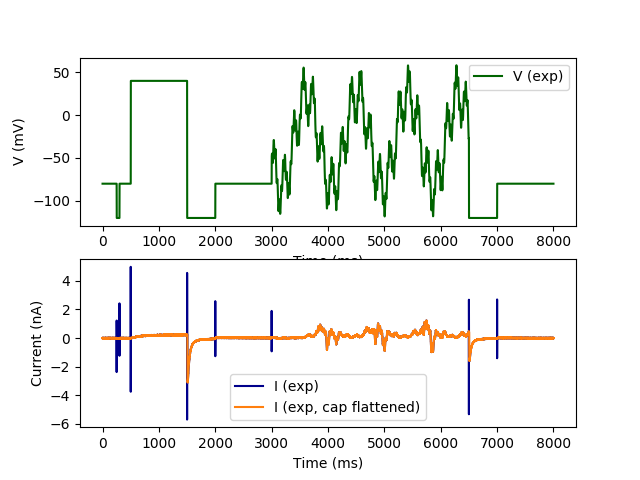
\includegraphics[width=0.75\textwidth]{fig/sine-wave-data}
}
\caption{%
Sine wave data shown uncorrected (blue, passed to modelling stage) and
 corrected (orange).
}
\label{fig:overview}
\end{figure}



\subsection{Simulating with Kylie's model}

Implemented Kylie's model in Myokit in two versions: one in Hodgkin-Huxley (HH)
 style (with two gating variables) and one in a Markov-model style (with four
 states $y_1$, $y_2$, $y_3$, $y_4$ where $y_{1,2,3}$ are described by ODEs
 while $y_4 = 1 - y_1 - y-2 - y_3$.
Used the \textbf{Markov} version throughout (to match Kylie's Matlab work).

\begin{verbatim}
IKr = p9 * y3 * (V - nernst.EK)
y4 = 1 - y1 - y2 - y3
k12 = p1 * exp( p2 * V)
k21 = p3 * exp(-p4 * V)
k41 = p5 * exp( p6 * V)
k14 = p7 * exp(-p8 * V)
dot(y1) = -k12 * y1 + k21 * y2 + k41 * y4 - k14 * y1
dot(y2) = -k14 * y2 + k41 * y3 + k12 * y1 - k21 * y2
dot(y3) = -k21 * y3 + k12 * y4 + k14 * y2 - k41 * y3
p1 = 2.26e-4 [1/ms]
p2 = 0.06990 [1/mV]
p3 = 3.45e-5 [1/ms]
p4 = 0.05462 [1/mV]
p5 = 0.08730 [1/ms]
p6 = 8.91e-3 [1/mV]
p7 = 5.15e-3 [1/ms]
p8 = 0.03158 [1/mV]
p9 = 0.15240 [mS/uF]
\end{verbatim}

Updated the Matlab code from GitHub to extract the parameters with more
 precision.
The results are given in \tab{kylies-parameters}.

\begin{table}[H]
\centering
\caption{Kylie's parameters}
\label{tab:kylies-parameters}
\startrowcolors
\footnotesize
\begin{tabular}{cccc}
\hline
\thead{Name} & \thead{Value} \\
\hline
$p_1$ & 2.26026076650526008e-04 \\
$p_2$ & 6.99168845608636041e-02 \\
$p_3$ & 3.44809941106439982e-05 \\
$p_4$ & 5.46144197845310972e-02 \\
$p_5$ & 8.73240559379589998e-02 \\
$p_6$ & 8.91302005497139962e-03 \\
$p_7$ & 5.15112582976275015e-03 \\
$p_8$ & 3.15833911359110001e-02 \\
$p_9$ & 1.52395993652347989e-01 \\
\hline
\end{tabular}
\end{table}

The protocol was implemented in Myokit in a two-step process..
First, voltage steps were applied using Myokit's step protcol functionality,
 using the steps given in \tab{sine-wave-steps}.

\begin{table}[H]
\centering
\caption{Voltage steps in sine wave protocol. Note the 0.1ms offset.}
\label{tab:sine-wave-steps}
\startrowcolors
\footnotesize
\begin{tabular}{cccc}
\hline
\thead{Start (ms)} & \thead{Duration (ms)} & \thead{Potential (mV)} \\
\hline
0       &   250.1   &   -80     \\
250.1   &   50      &   -120    \\
300.1   &   200     &   -80     \\
500.1   &   1000    &   40      \\
1500.1  &   500     &   -120    \\
2000.1  &   1000    &   -80     \\
3000.1  &   3500    &   -30     \\
6500.1  &   500     &   -120    \\
7000.1  &   1000    &   -80     \\
\hline
\end{tabular}
\end{table}

Secondly, the model was amended to switch between the step protocol
 (represented by the variable \code{engine.pace}) and a sine wave:

\begin{verbatim}
model.get('membrane.V').set_rhs(
    'if(engine.time >= 3000.1 and engine.time < 6500.1,'
    + ' - 30'
    + ' + 54 * sin(0.007 * (engine.time - 2500.1))'
    + ' + 26 * sin(0.037 * (engine.time - 2500.1))'
    + ' + 10 * sin(0.190 * (engine.time - 2500.1))'
    + ', engine.pace)')
\end{verbatim}

At this point, capacitance filtering was also applied, using a similar strategy
 to Kylie's code, in which data points from the first 5ms after each voltage
 transition were removed from the data set used to perform fitting.
For example, given a time series $(t_1, x_1), (t_2, x_2), ..., (t_n, x_n)$
 such a filter could omit all data from $t_{11}$ to $t_{15}$, resulting in the
 filtered series
 $(t_1, x_1), (t_2, x_2), ..., (t_{10}, 10_{x}), (t_{16}, x_{16}), ..., (t_n, x_n)$.
Alternative strategies, such as setting $x_{11}, x_{12}, ..., x_{15}$ to some
 estimated value (e.g. zero) all require some assumptions to be made, so simply
 ignoring these data points is the simplest and safest option.

\subsubsection{Solver settings}

Solver tolerances were set to $10^{-8}$, $10^{-8}$, to match Kylie's
 simulations.
Note that the the tolerances are checked w.r.t. the states, not the output
 variable \ikr.
Since the states $y_i \leq 1$, the relative tolerance is usually the more
 stringent of the two.
Since \ikr\ is between 0 and 120 times $g$ ($\approx 0.1$) times $y_3$, it
 seems the error in \ikr\ will be between 0 and 12 times that in $y_3$ so
 $O(10^{-7})$.
Finally, this is a per-step tolerance, not a global tolerance.
A a rule of thumb, The CVODE manual suggests setting the tolerance to 0.01
 times the desired global tolerance, suggesting an error of $O(10^{-5})$ in
 \ikr\ might be accepted.

Both Myokit and Kylie's code use the \code{CV\_BDF} and \code{CV\_NEWTON}
 methods.
A difference between the Myokit simulation and the one used by Kylie is that
 Myokit resets the solver at each voltage step transition (but not during the
 sine wave protocol).
The advantage of this method is that you don't need to set a maximum step size
 (Kylie's simulation uses a max step size of $0.1$ms).

The Matlab code makes repeated calls (one for each $0.1$ms interval) to CVODE,
 using the \code{CV\_NORMAL} calling mode.
This asks the solver to step \emph{to or just over} the next point in time, and
 returns the value at the requested time via interpolation.
Note that this is independent of the maximum step size, so in the Matlab code
 the solver might move from $t=0$ms to $t=1$ms via the points $0$ms, $0.7$ms,
 $1.7$ms with an interpolation to get the result at $t=1$ms.
The Myokit code makes calls using the \code{CV\_ONE\_STEP} mode, which makes
 steps of an arbitrary length.
As soon as the next logging point is passed, Myokit then asks CVODE to return
 the values at the desired time via interpolation.
Because no maximum step size is given, the example above could become $0$ms,
 $0.7$ms, $2.4$ms with an interpolation to get the result at $t=1$ms.
So in effect both methods step to arbitrary points beyond the next requested
 time and then deliver an answer using interpolation.

The major difference between the two methods are that (1) Myokit regularly
 resets the solver, causing small steps to be made just after each transition
 and (2) the Matlab code enforces a maximum step size of $1$ms.

\subsubsection{How well do the Matlab/Myokit protocol implementations match?}

To check how well the Myokit protocol matched the Matlab one, I compared
 against Kylie's protocol files.
Because the data supplied on GitHub was used to generate figures and didn't
 show all digits used internally, I generated new files with higher precision
 output.
\Fig{sine-wave-protocol-error} shows the difference in the membrane potential
 between the resulting Matlab protocol file and the membrane potential
 simulated in Myokit.
Some error still occurs during the sine-wave, but this is on the order of
 numerical error (typically given as $O(10^{15}$) for double precision).

\begin{figure}[H]
\centerline{
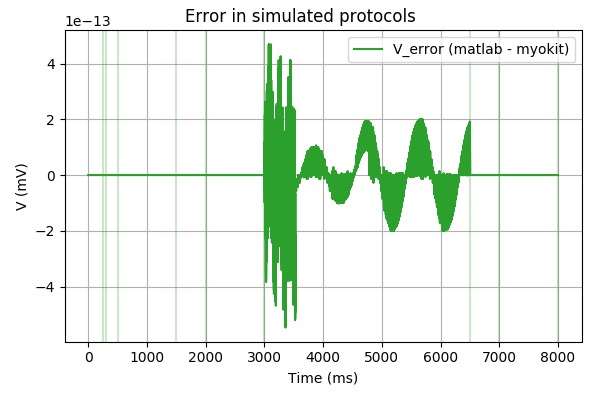
\includegraphics[width=0.75\textwidth]{fig/sine-wave-protocol-error}
}
\caption{%
Difference between the Matlab and Myokit implementations of the voltage
 protocol.
The maximum difference at any moment in time is 6e-13 mV.
}
\label{fig:sine-wave-protocol-error}
\end{figure}

\subsubsection{And what about the simulations?}

To check simulation results, I extracted new high-precision data files from the
 Matlab implementation and plotted them in \fig{sine-wave-current-error-tol8}.
At first glance, the difference between the implementations seems to be
 relatively large.

\begin{figure}[H]
\centerline{
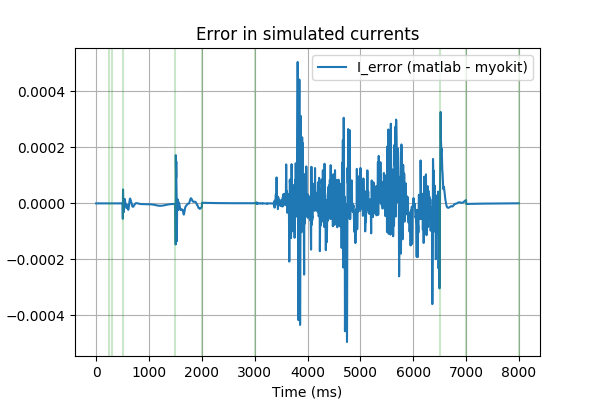
\includegraphics[width=0.75\textwidth]{fig/sine-wave-current-error-tol8}
}
\caption{%
Difference between the Matlab and Myokit simulations of current during the
 voltage protocol, both with tolerances of $10^-8$.
The same capacitance filtering was applied to both traces.
The maximum difference at any moment in time is 5e-4 nA.
}
\label{fig:sine-wave-current-error-tol8}
\end{figure}

To check if this was due to a difference in the model, or simply an
 accumulation of small numerical differences, I re-ran \emph{both simulations}
 with higher tolerances ($10^{-10}$, $10^{-10}$).
The result is shown in \fig{sine-wave-current-error-tol10}.

This $10^4$ increase in precision after a $10^2$ increase in tolerance suggests
 that the errors in the signals are not systematic.

\begin{figure}[H]
\centerline{
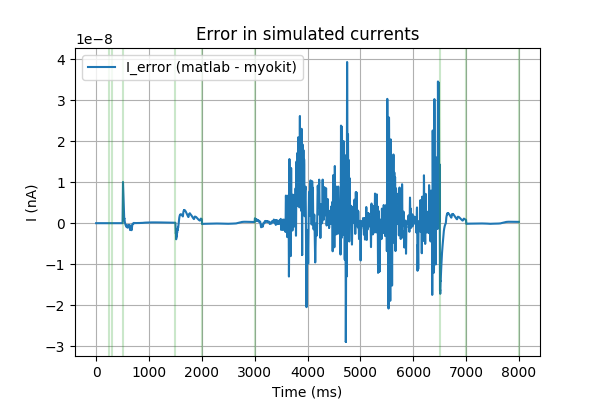
\includegraphics[width=0.75\textwidth]{fig/sine-wave-current-error-tol10}
}
\caption{%
Difference between the Matlab and Myokit simulations of current during the
 voltage protocol, both with tolerances of $10^-10$.
The same capacitance filtering was applied to both traces.
The maximum difference at any moment in time is 4e-8 nA.
}
\label{fig:sine-wave-current-error-tol10}
\end{figure}

Adding a maximum step size of $0.1$ reduces the difference further, as seen in
 \fig{sine-wave-current-error-tol10-max-step}.

\begin{figure}[H]
\centerline{
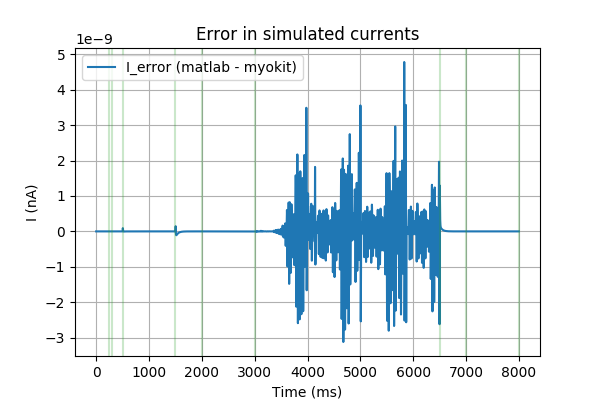
\includegraphics[width=0.75\textwidth]{fig/sine-wave-current-error-tol10-max-step}
}
\caption{%
Difference between the Matlab and Myokit simulations of current during the
 voltage protocol, both with tolerances of $10^-10$ and a maximum step size of
 $1.0$ms.
The same capacitance filtering was applied to both traces.
The maximum difference at any moment in time is 5e-9 nA.
}
\label{fig:sine-wave-current-error-tol10-max-step}
\end{figure}

It seems that the difference at this point is largely due to the difference in
 the input protocol.



\subsubsection{Log-likelihood calculation}

I next calculated the log-likelihood of the data, given Kylie's parameters and
 stochastic gaussian noise.
The standard deviation of the noise was determined as the standard deviation
 of the first 200ms (2000 samples) of data, and is given in
 \tab{sine-wave-noise}.

\begin{table}[H]
\centering
\caption{Noise in the first 200ms.}
\label{tab:sine-wave-noise}
\startrowcolors
\footnotesize
\begin{tabular}{c}
\hline
\thead{$\sigma_\text{noise}$ (nA)}  \\
\hline
0.00462852386082 \\
\hline
\end{tabular}
\end{table}

The log-likelihood was then calculated using Pints (and Myokit for simulations)
 and compared with a value calculated with a simplified version of Kylie's
 Matlab code (on another machine).
Both results are shown in \tab{sine-wave-loglikelihood}.

\begin{table}[H]
\centering
\caption{%
Log-likelihood of Cell 5 data given Kylie's cell 5 parameters.
Pints/Myokit vs. Matlab.
All calculated with $10^-10$ solver tolerances (but on separate machines).
}
\label{tab:sine-wave-loglikelihood}
\startrowcolors
\footnotesize
\begin{tabular}{ll}
\hline
\thead{Method} & \thead{Log-likelihood} \\
\hline
Pints/Myokit & -1.510 4 1629778709938e+06 \\
Matlab       & -1.510 6 37413819120  e+06 \\
\hline
\end{tabular}
\end{table}

I found a couple of reasons for this difference.
(1) Matlab and NumPy have different defaults for the \code{std()} function.
In particular, Matlab uses the unbiased $1/(n-1)$ estimation by default, which Python does not.
(2) Kylie's capacitance filtering different very slightly from mine, starting 2 samples earlier and finishing 1 sample earlier.
In addition, Kylie doesn't filter at the start of the sine wave.
(3) Kylie's code performed a log10 transform, and then undid it again, leading to slightly different parameters.
(4) As seen in the graphs above, the simulation data differs slightly between the Matlab and Myokit implementations.

\Tab{sine-wave-loglikelihood2} shows the \emph{cumulative} effect of
 compensating for these differences.
The top row shows the original results from \tab{sine-wave-loglikelihood}.
In the next row, Python is made to use a similar sample standard deviation
 calculation is Matlab.
This appears to make things worse.
However, the next row shows that if the capacitance filtering is also changed,
 the results grow much closer.
Similarly, applying \emph{only} the capacitance filtering change led to a worse
 result.
In the 4th row, the Python code is made to perform a log10 transform and
 detransform.
After this operation, the results agree to within 10 digits.

The final row shows the effects of omitting the Myokit simulations altogether.
Interestingly, this still only gives 10 digits precision.
Factors that might explain this final difference are:
(1) Different implementations of numerical operators between Python/Matlab.
(2) Differences in data loading between Matlab and Python
(3) Differences between the machines the tests were run on.

\begin{table}[H]
\centering
\caption{%
An exploration of the differences in \tab{sine-wave-loglikelihood}.
}
\label{tab:sine-wave-loglikelihood2}
\startrowcolors
\footnotesize
\begin{tabular}{ll}
\hline
\thead{Method} & \thead{Log-likelihood} \\
\hline
Pints/Myokit        & -1.510 4 1629778709938e+06 \\
Matlab              & -1.510 6 37413819120  e+06 \\
\hline
+fix std()          & -1.5 0 950362278065225e+06 \\
Matlab              & -1.5 1 0637413819120  e+06 \\
\hline
+fix cap filter     & -1.51063741 5 35030073e+06 \\
Matlab              & -1.51063741 3 819120  e+06 \\
\hline
+log10 transform    & -1.510637413 2 5626755e+06 \\
Matlab              & -1.510637413 8 19120  e+06 \\
\hline
+kylie's data      & -1.510637413 3 1823613e+06 \\
Matlab              & -1.510637413 8 19120  e+06 \\
\hline
\end{tabular}
\end{table}

Following up on the observation that the forward and backward $\log10$
 transform makes a difference, I ran one more simulation with the
 transformed/untransformed parameters, shown in
 \fig{sine-wave-current-error-tol10-max-step-transform}.

\begin{figure}[H]
\centerline{
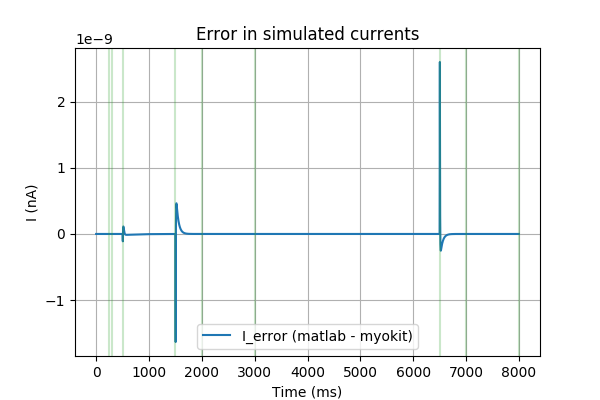
\includegraphics[width=0.75\textwidth]{fig/sine-wave-current-error-tol10-max-step-transform}
}
\caption{%
Difference between the Matlab and Myokit simulations of current during the
 voltage protocol, both with tolerances of $10^{-10}$, a maximum step size of
 $1.0$ms, and the parameters transformed and untransformed.
The same capacitance filtering was applied to both traces.
The maximum difference at any moment in time is 3e-9 nA.
}
\label{fig:sine-wave-current-error-tol10-max-step-transform}
\end{figure}

As seen, this completely removes the error during the sine-wave part, leading
 only to differences at the voltage transitions (indicated with vertical green
 lines).

\subsection{Conclusions}

\begin{enumerate}
\item Simulating in Matlab and Myokit gives similar log likelihoods.
\item Differences in capacitance filtering and the \code{std()} method can lead
 to $O(10^{-4})$ differences in the calculated log-likelihood.
\item Because $O(10^{-4})$ isn't all that big, we should be able to continue
 using the methods used to create \tab{sine-wave-loglikelihood} (so Python
 \code{std()} and slightly different capacitance filtering from Kylie)
\end{enumerate}










%
%
% CMA-ES
%
%
\section{Finding the optimal parameters}

Set up CMAES fitting in Pints, using the same model implementation as in the
 previous section.
But: this time with tolerances $10^-8$ and without the minimum step size.

\subsection{Prior / boundaries / constraints}

Kylie's model uses three types of constraint.

The first is a manually determined lower and upper bound on the conductance
 parameter ($p_9$).

The remaining eight parameters are divided into \emph{a}s
 ($p_1, p_3, p_5, p_7$) and \emph{b}s ($p_2, p_4, p_6, p_8$).
Each rate constant then has the form $r_i = a_j \exp(b_k V)$.
The second constraint is:
\begin{align*}
10^{-7} < a < 10^3 \\
10^{-7} < b < 0.4 \\
\end{align*}

The third constraint is on the rate parameters and on the the applied voltage
 V.

\begin{align*}
r1 &= p_1 \exp(p_2 V) \\
r2 &= p_3 \exp(-p_4 V) \\
r3 &= p_5 \exp(p_6 V) \\
r4 &= p_7 \exp(-p_8 V)
\end{align*}

This constraint says that \emph{the maximum rate during the protocol} must
 be within certain physiological bounds.
The minimum rate is unbounded (but $\geq 0$ due to the previous constraints on
 the \emph{a}s and \emph{b}s).

\begin{align*}
r_\text{min} &< \max_{V \in \{V_\text{min}, V_\text{max}\}} r(V) < r_\text{max} \\
r_\text{min} &= 1.67 \cdot 10^{-5} \text{ms}^{-1} \\
r_\text{max} &= 1000 \text{ms}^{-1} \\
V_\text{min} &= -120 \text{mV} \\
V_\text{max} &= 58.25 \text{mV}
\end{align*}


For the forward rates, $r_1$ and $r_3$ we find

\begin{align}
\max\{ a e^{b V_\text{min}}, a e^{b V_\text{max}} \} &> r_\text{min} \\
a e^{b V_\text{max}} &> r_\text{min} \\
b &> \frac{\log r_\text{min} - \log a}{V_\text{max}}, \qquad V_\text{max} > 0
\end{align}
and
\begin{align}
\max\{ a e^{b V_\text{min}}, a e^{b V_\text{max}} \} &< r_\text{max} \\
a e^{b V_\text{max}} &< r_\text{max} \\
b &< \frac{\log r_\text{max} - \log a}{V_\text{max}}, \qquad V_\text{max} > 0
\end{align}

For the backward rates, $r_2$ and $r_4$ we find

\begin{align}
\max\{ a e^{-b V_\text{min}}, a e^{-b V_\text{max}} \} &> r_\text{min} \\
a e^{-b V_\text{min}} &> r_\text{min} \\
b &> \frac{\log r_\text{min} - \log a}{V_\text{min}}, \qquad V_\text{min} < 0
\end{align}
and
\begin{align}
\max\{ a e^{-b V_\text{min}}, a e^{-b V_\text{max}} \} &< r_\text{max} \\
a e^{-b V_\text{min}} &< r_\text{max} \\
b &< \frac{\log r_\text{max} - \log a}{V_\text{min}}, \qquad V_\text{min} < 0
\end{align}

So the forward rates are bound by $V_\text{max}$ and the backward rates are bound by
$V_\text{min}$.

\begin{figure}[H]
\centerline{
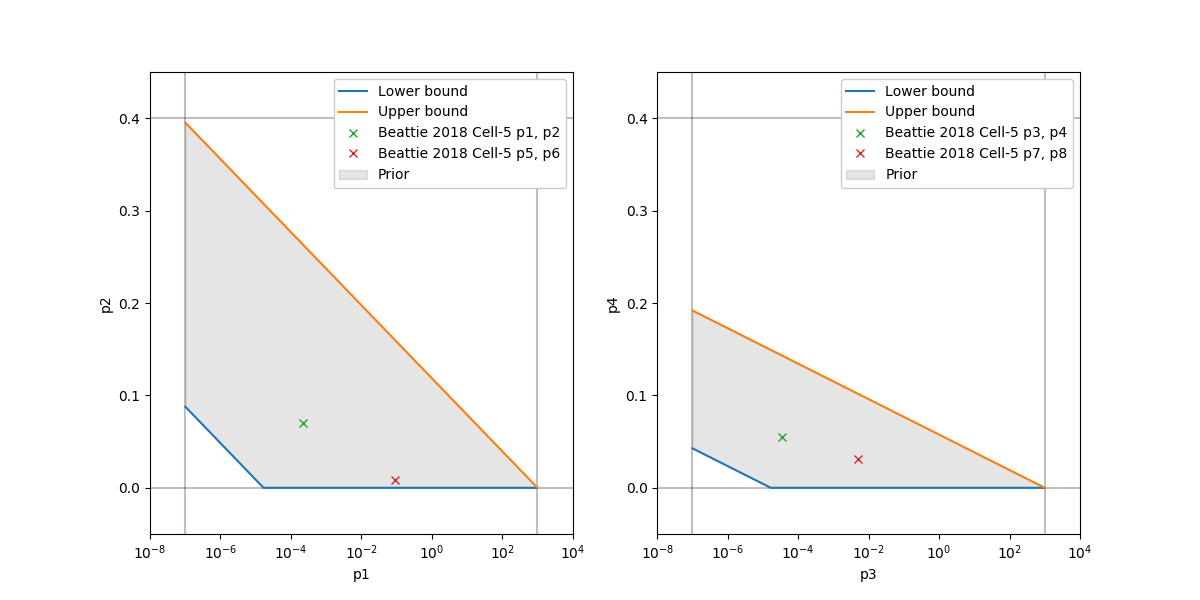
\includegraphics[width=0.95\textwidth]{fig/prior}
}
\caption{%
Prior on forward rates (left) and backward rates (right).
}
\label{fig:prior}
\end{figure}

The full prior is then created by combining the constants on $a$s, $b$s, and
 $r$s for each rate, and finally adding a lower and upper bound on the
 conductance.
Values for the conductance bounds are taken from Kylie's code without
 modification.

Note: At the time of writing it seems that the Matlab code in the sine wave
 project only checks the rate constant constraints for the fastest rate in
 the model.
This means that the upper bounds in \fig{prior} are enforced, but the lower
 bounds (from the rate constants, the diagonal bit in the bottom left corner)
 are only enforced for the fastest rate.
In other words, some values are allowed end up in the little white triangle in
 the bottom left corner.
This will be fixed soon, but shouldn't change the results as the current values
 are within the grey shaded area.


\subsection{Selecting starting points}

To run an optimisation, we need to select some starting points within the
 prior.
Sampling within the boundaries on the parameters themselves is easy: just
 collect all lower and upper bounds and sample a 9d parameter vector uniformly
 within those bounds.
However, this doesn't guarantee it meets the rate constant constraints.

The simplest strategy to deal with this is to do rejection-sampling
 (accept-reject): Sample points within the parameter boundaries, then check if
 they violate the rate constant constraints, and if so, reject them and sample
 again.
If we sample a 9d point uniformly within the outer bounds, the chances of
 getting a point that meets the rate constant requirements are not good.
\Fig{prior-no-log} shows the prior in an untransformed space.
The area's of the grey areas are approximately 0.043 (forward) and 0.021
 (backward) times the area of the parameter bounds.
This means that testing a single sample with two forward and two backward
 rates the chances of acceptance are approximately
 $0.043^2 \cdot 0.021^2 \approx 8.2 \cdot 10^-7$, so that an average of 1 in
 1.2 million samples would be accepted.

Kylie's Matlab code gets around this by sampling uniformly in a much smaller
 space, with boundaries close to the minimum and maximum values found in models
 in the literature.

However, if we log transform the $a$ parameters, our chances get much better.
From \fig{prior} we can estimate the forward area is $\approx 0.5$ times the
 total area, while the backward area is approx $0.25$ times the total area.
To further improve our chances we can split the problem into 5 subproblems:
 Twice sampling the parameters for a forward rate, twice sampling the
 parameters for a backward rate, and finally sampling a conductance value.
This should raise our sampling success rate, leading to an expected number of
 2 + 2 + 4 + 4 = 12 samples needed to get a single accepted 9d point.

\begin{figure}[H]
\centerline{
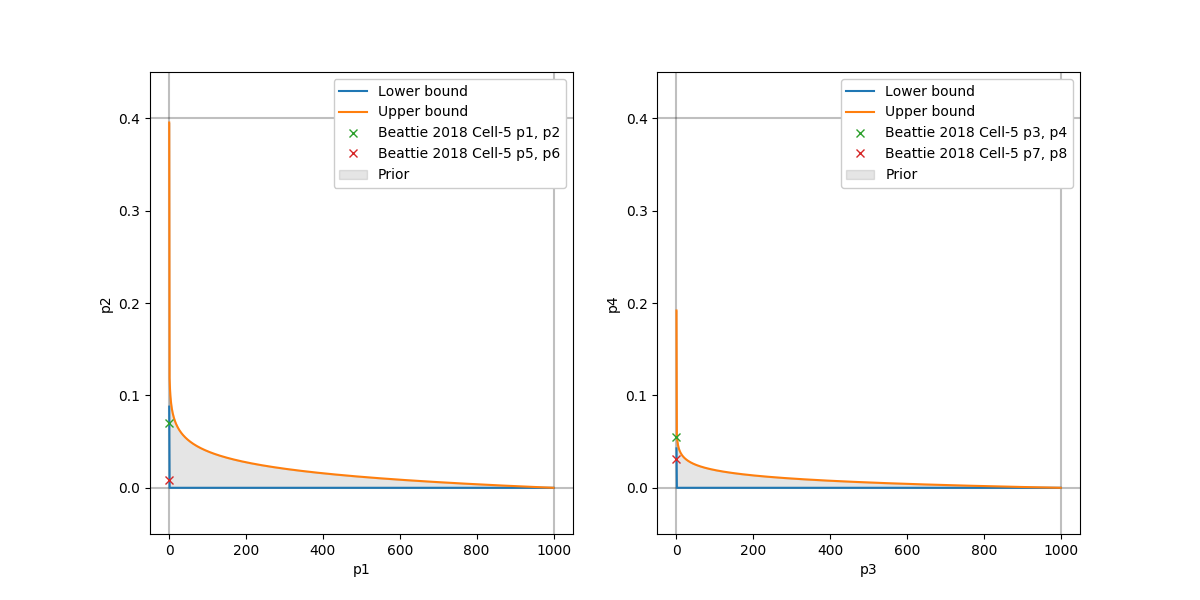
\includegraphics[width=0.95\textwidth]{fig/prior-no-log}
}
\caption{%
Prior on forward rates (left) and backward rates (right), shown without a
logarithmic axes for $p_1$, $p_5$, $p_3$ and $p_7$.
}
\label{fig:prior-no-log}
\end{figure}


\subsection{Running an optimisation}

Using Pints, which wraps around CMA-ES (as well as providing other
 optimisation algorithms and MCMC).
Created a \code{KnownNoiseLogLikelihood} using a $\sigma$ estimated from the
 first 2000 data points (200ms, when the signal is flat).
To estimate it, I used the sample standard deviation with ddof=1 (the $n - 1$
 version).
Then added a custom \code{LogPrior} object that implemented the parameter and
 rate constraints (as well as providing the sampling method described above).
Combined these into a \code{LogPosterior} and passed that to the
 \code{Optimisation} class (which maximises it).
Because the \code{LogPrior} evaluates to $-\infty$ when the constraints are
 violated, the problem is automatically bounded and so no \code{Boundaries}
 object was passed to the optimiser.
Evaluation of the \code{LogPosterior} (which involves a simulation) was set to
 happen in parallel.
CMAES was chosen as the optimisation method.

As stopping criteria we used the occurrence of 200 subsequent iterations
 without a significant change in the score function (threshold 1e-11).
No other stopping criteria were applied.

The fits were then run on scrambler, which provides 24 real and 24 fake cores
 (hyperthreading), allowing 48 simulations to be run in parallel(ish,
 hyperthreading).
A population size of 48 was used, leading to a core use of approx 80\% each
 (perhaps we should double/triple the population size?).
With these settings, scrambler runs around 4 iterations per second.
25 repeats were run (sequentially), all from different points sampled from the
 prior.

\subsection{Results}

Results from CMAES were highly similar to those found by Kylie.

\begin{table}[H]
\centering
\caption{%
Results of parameter fitting, compared with published results by Kylie.
The log-likelihoods shown were calculated using Myokit/Pints, in exactly the
same manner but with a different parameter set.
}
\label{tab:sine-wave-loglikelihood2}
\startrowcolors
\footnotesize
\begin{tabular}{lll}
\hline
\thead{Value} & \thead{Kylie} & \thead{Myokit/Pints} \\
\hline
$p_1$ & 2.26 026076650526008e-04 & 2.26 137846758451367e-04 \\
$p_2$ & 6.991 68845608636041e-02 & 6.991 30764903859586e-02 \\
$p_3$ & 3.44 809941106439982e-05 & 3.44 958226788683007e-05 \\
$p_4$ & 5.461 44197845310972e-02 & 5.461 21826895913237e-02 \\
$p_5$ & 8.7324 0559379589998e-02 & 8.7324 2841545401188e-02 \\
$p_6$ & 8.9 1302005497139962e-03 & 8.9 3017989292029316e-03 \\
$p_7$ & 5.1 5112582976275015e-03 & 5.1 4883265963462632e-03 \\
$p_8$ & 3.15 833911359110001e-02 & 3.15 620982414665449e-02 \\
$p_9$ & 1.52 395993652347989e-01 & 1.52 436968881218465e-01 \\
log-likelihood & -1.509 50112826760067e+06 & -1.509 48474675446958e+06 \\
\hline
\end{tabular}
\end{table}







%
%
% MCMC
%
%
\section{Inferring a distribution around the optimal parameters}

Started MCMC using adaptive covariance MCMC.
3 chains in parallel using Pints.
All starting from position found by CMAES.
Ran for 250 000 iterations, discarded first 50 000 as warm-up.
No thinning was applied.

Inspected results of 3 chains: All kept to highly similar mean, found highly
 similar distribution.
Continued analysis with only 1st chain.

\begin{figure}[H]
\centerline{
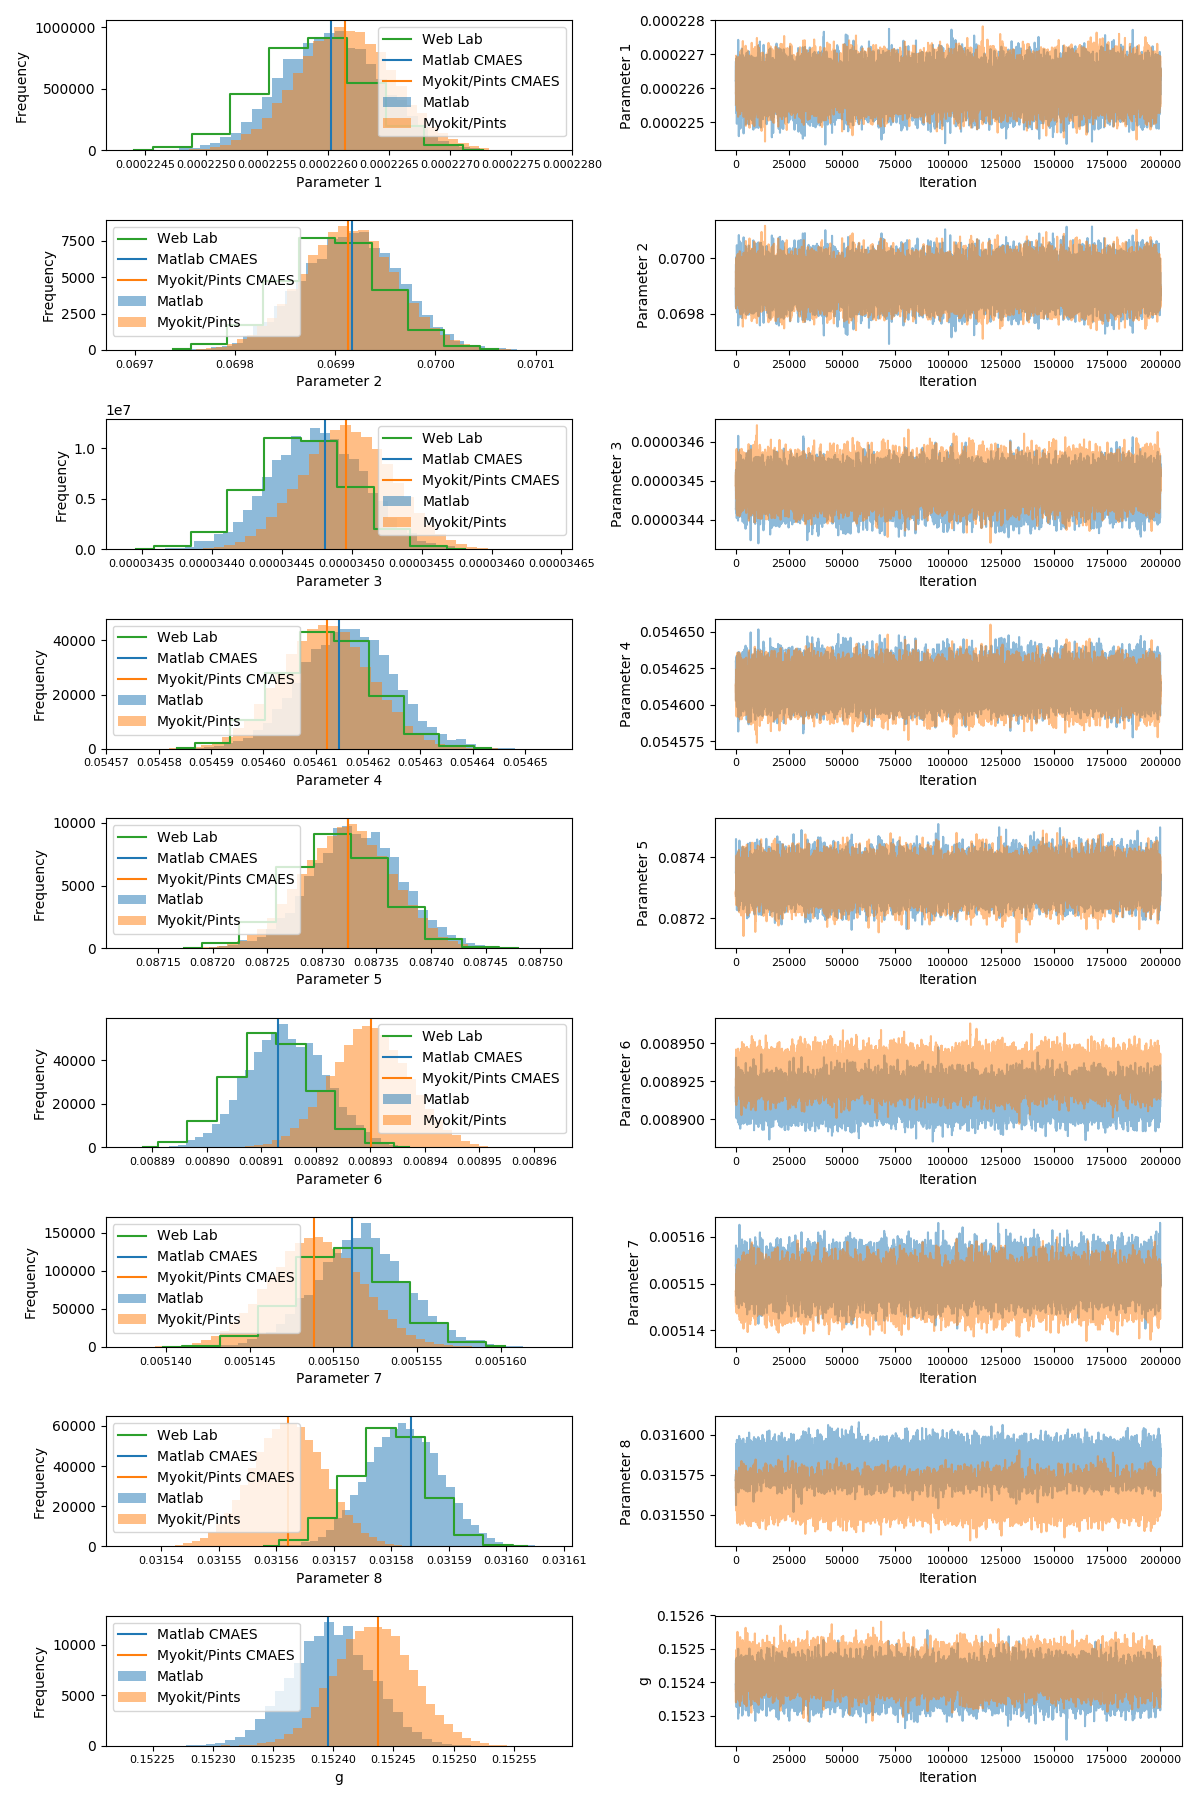
\includegraphics[width=0.95\textwidth]{fig/sine-wave-mcmc-trace}
}
\caption{%
MCMC results comparison, Matlab, Web Lab, Pints/Myokit.
The resulting distributions all have similar widths, but there are very slight
 (3d decimal) shifts in the means for some parameters.
Plotting the CMAES results (vertical lines) reveals these small shifts are due
 to the same factors identified for the CMAES results.
}
\label{fig:sine-wave-mcmc-trace}
\end{figure}


\begin{figure}[H]
\centerline{
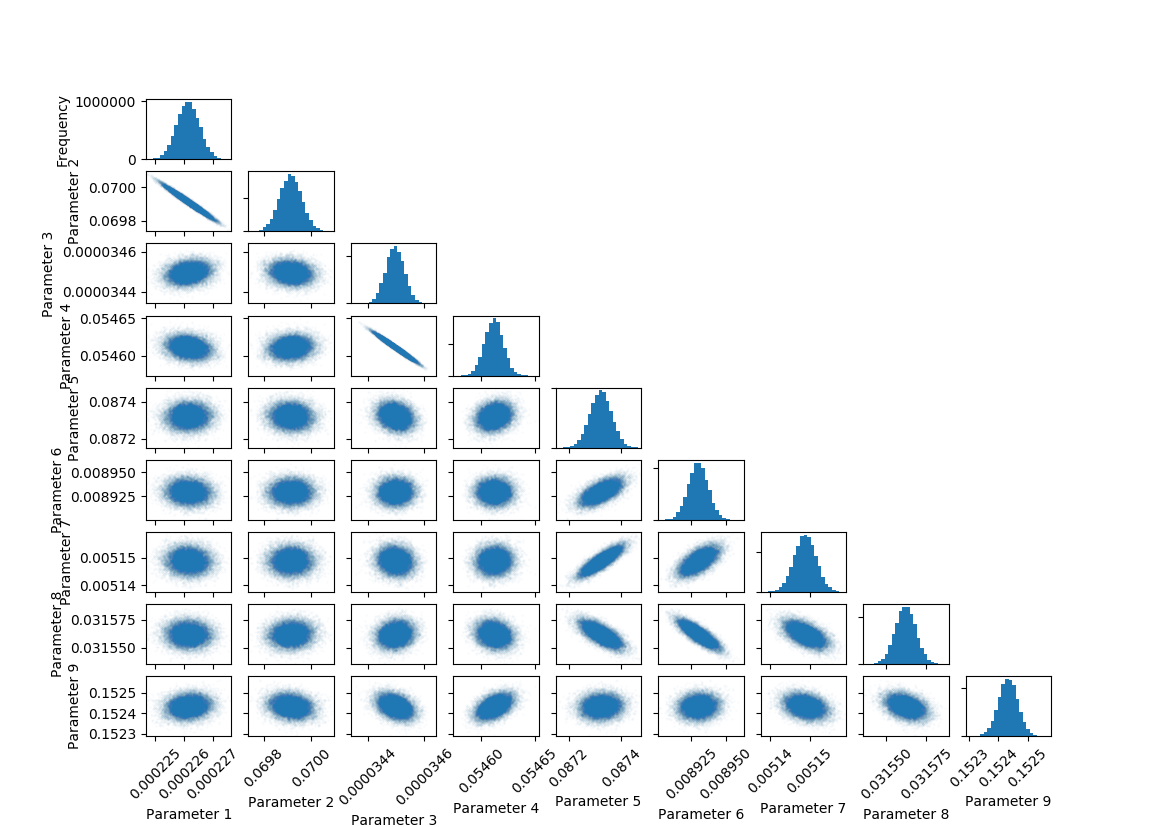
\includegraphics[width=0.95\textwidth]{fig/sine-wave-mcmc-pairwise}
}
\caption{%
Pairwise plots of correlations between parameter values, as found by MCMC.
}
\label{fig:sine-wave-mcmc-pairwise}
\end{figure}





%
%
% Traditional protocols
%
%
\section{Fitting to multiple traces / Traditional protocols}

Loaded the first activation protocol ("steady activation").
Again, the first step has one extra time point: adjusted the simulation
protocol to match this.
Results of importing the data shown in \fig{steady-activation}.
Ran simulations with the parameters Kylie inferred from the sine wave
 experiments.
The error between the simulated and measured current is considerable.

\begin{figure}[H]
\centerline{
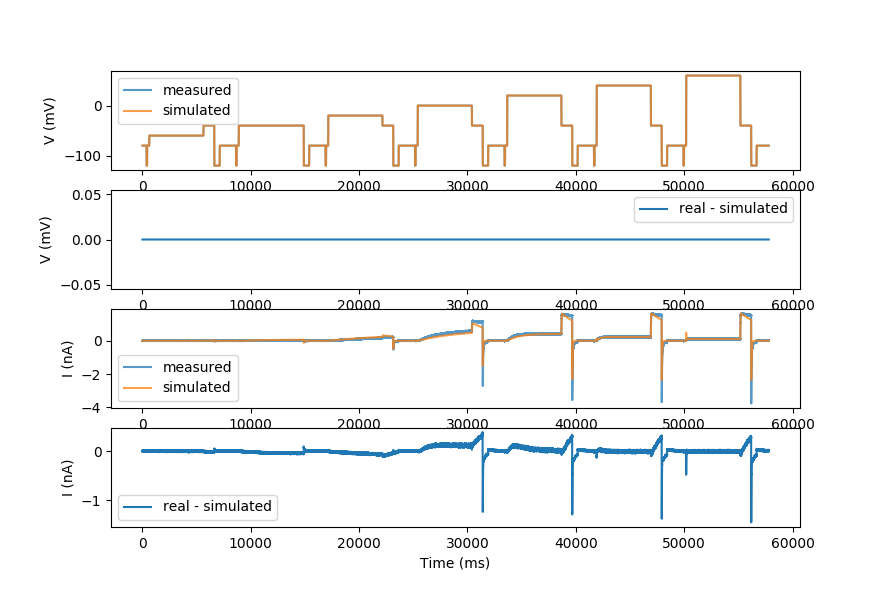
\includegraphics[width=0.75\textwidth]{fig/activation-1-data-and-sim}
}
\caption{%
The first activation protocol (steady activation): data and simulation with
Kylie's parameters from the sine-wave protocol.
}
\label{fig:steady-activation}
\end{figure}

\begin{figure}[H]
\centerline{
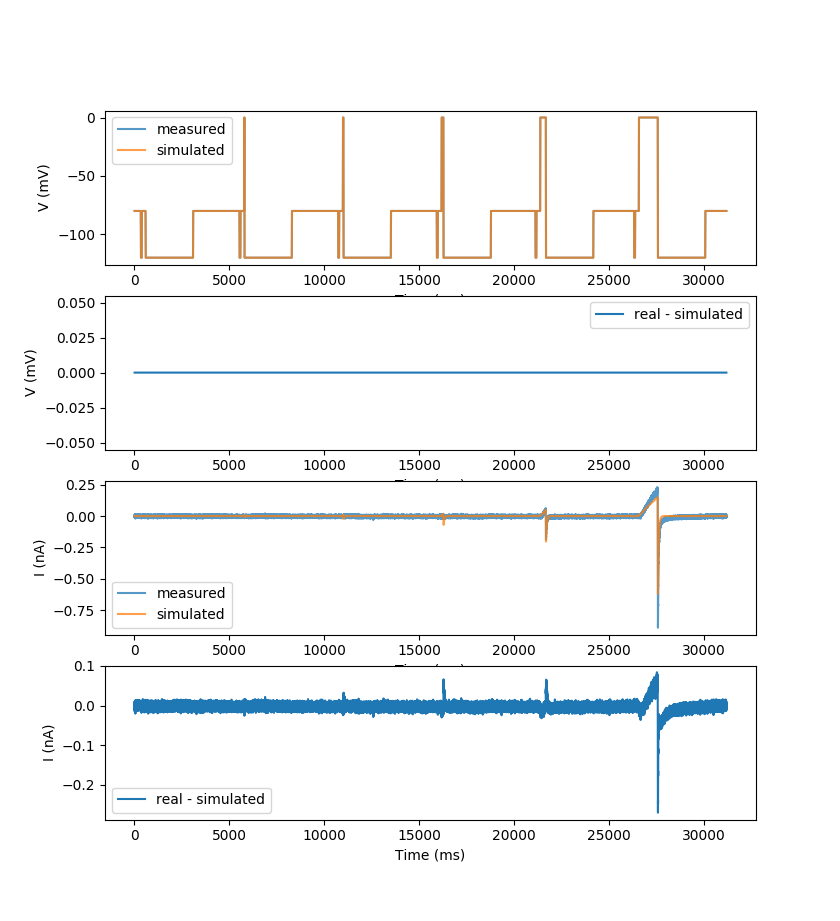
\includegraphics[width=0.75\textwidth]{fig/activation-2-data-and-sim}
}
\caption{%
The second activation protocol (activation kinetics 1): data and simulation
with Kylie's parameters from the sine-wave protocol.
}
\label{fig:activation-kinetics-1}
\end{figure}

\begin{figure}[H]
\centerline{
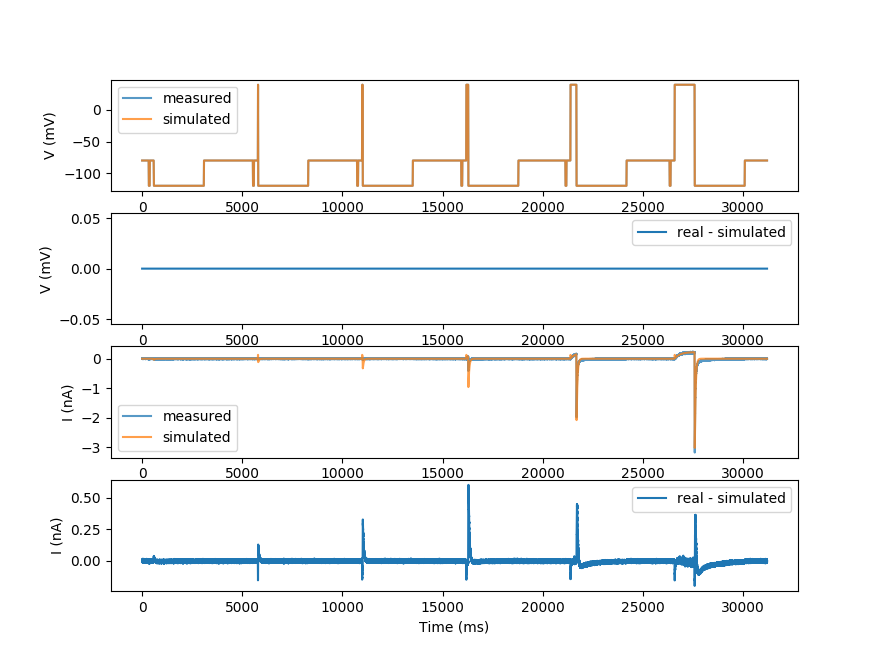
\includegraphics[width=0.75\textwidth]{fig/activation-3-data-and-sim}
}
\caption{%
The third activation protocol (activation kinetics 2): data and simulation
with Kylie's parameters from the sine-wave protocol.
}
\label{fig:activation-kinetics-2}
\end{figure}

\begin{figure}[H]
\centerline{
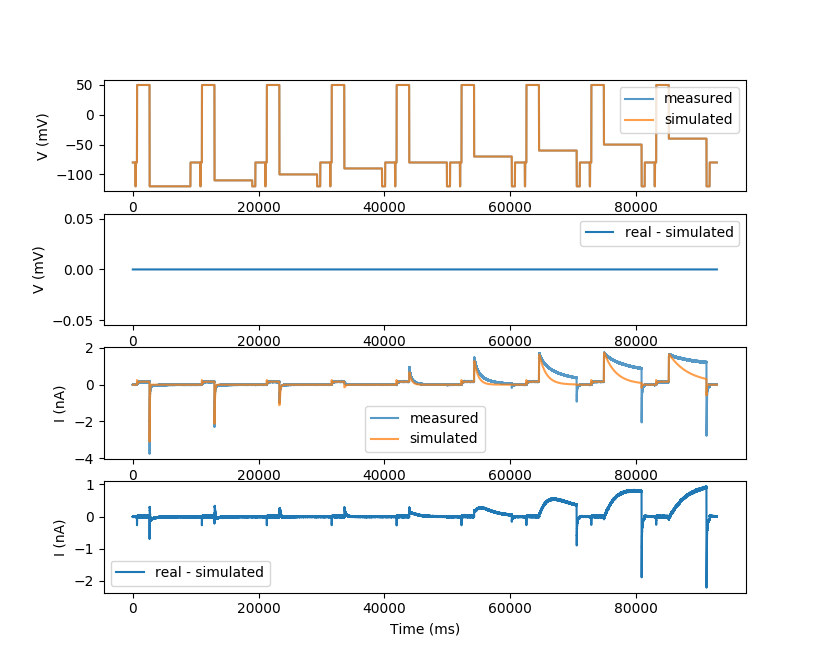
\includegraphics[width=0.75\textwidth]{fig/deactivation-data-and-sim}
}
\caption{%
The deactivation protocol: data and simulation with Kylie's parameters from the
sine-wave protocol.
}
\label{fig:deactivation}
\end{figure}

\begin{figure}[H]
\centerline{
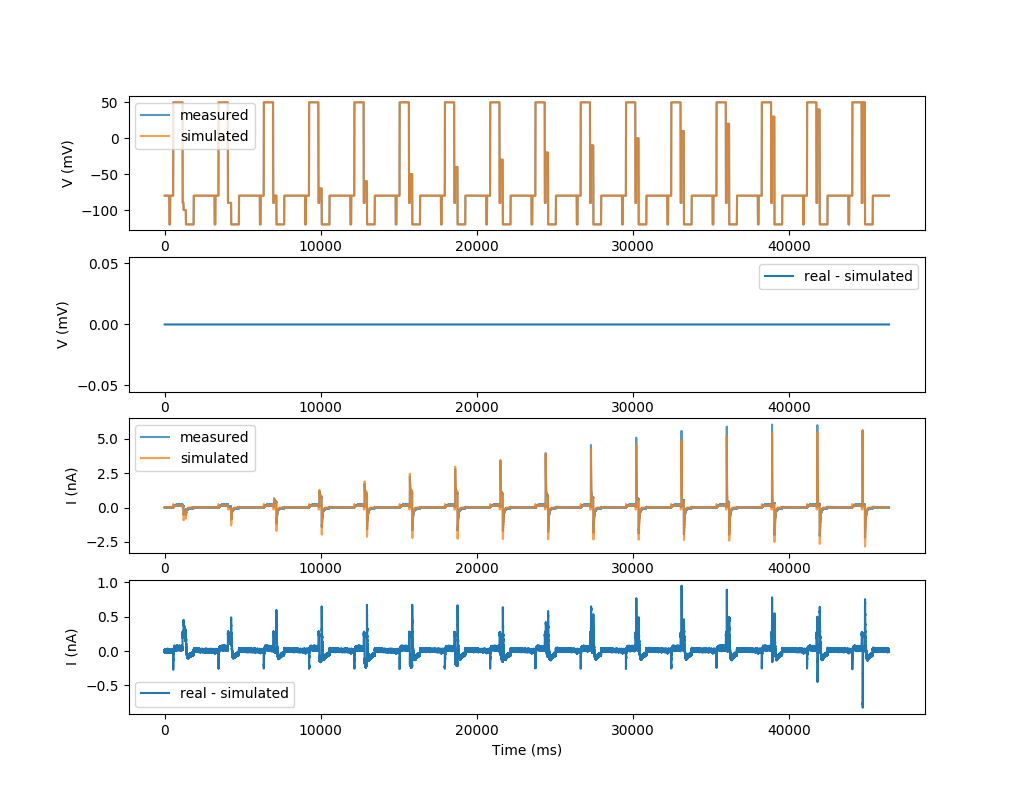
\includegraphics[width=0.75\textwidth]{fig/inactivation-data-and-sim}
}
\caption{%
The inactivation protocol: data and simulation with Kylie's parameters from the
sine-wave protocol.
}
\label{fig:inactivation}
\end{figure}



\subsection{Fitting to trad. prot.}




\begin{table}[H]
\centering
\caption{%
Results of parameter fitting, comparing sine wave results with results from
fitting to whole traces using traditional protocols.
}
\label{tab:sine-wave-loglikelihood2}
\startrowcolors
\footnotesize
\begin{tabular}{lll}
\hline
\thead{Value} & \thead{Sine wave} & \thead{Traditional traces} \\
\hline
$p_1$ & 2.261e-4 & 2.364e-4 \\
$p_2$ & 6.991e-2 & \textbf{7}.563e-2 \\
$p_3$ & 3.450e-5 & 3.313e-\textbf{6} \\
$p_4$ & 5.461e-2 & \textbf{7}.391e-2 \\
$p_5$ & 8.732e-2 & \textbf{9}.255e-2 \\
$p_6$ & 8.930e-3 & 8.508e-3 \\
$p_7$ & 5.149e-3 & \textbf{6}.648e-3 \\
$p_8$ & 3.156e-2 & 3.098e-2 \\
$p_9$ & 1.524e-1 & 1.292e-1 \\
\hline
\end{tabular}
\end{table}





\subsection{MCMC on trad. prot.}

MCMC with same settings as previously.
Runs into some issues without an initial covariance set.
Had to use $I \cdot x_0 \cdot 10^{-35}$ to get any acceptance in the early
 stages.
Seems very very tight, presumably due to massive number of samples.













%
%
% Summary statistics
%
%
\section{Fitting to summary statistics}

Analysing 5 protocols.

Versions used so far match \emph{exactly} with the recorded signals, but have a
 few annoying issues with e.g. an extra sample added to the first step, or very
 slight variations in step size.
Figures below show simulation-only results with `tidied up' versions of same
 protocols.
Simulations are performed with fitting results to combined whole traces for
 these protocols.


%
% Pr1 and Pr2
%
\subsection{Pr1 and Pr2: Activation kinetics}

Pr1 and Pr2 differ only in size of one step.

% Analysis Pr1
\begin{figure}[H]
\centerline{
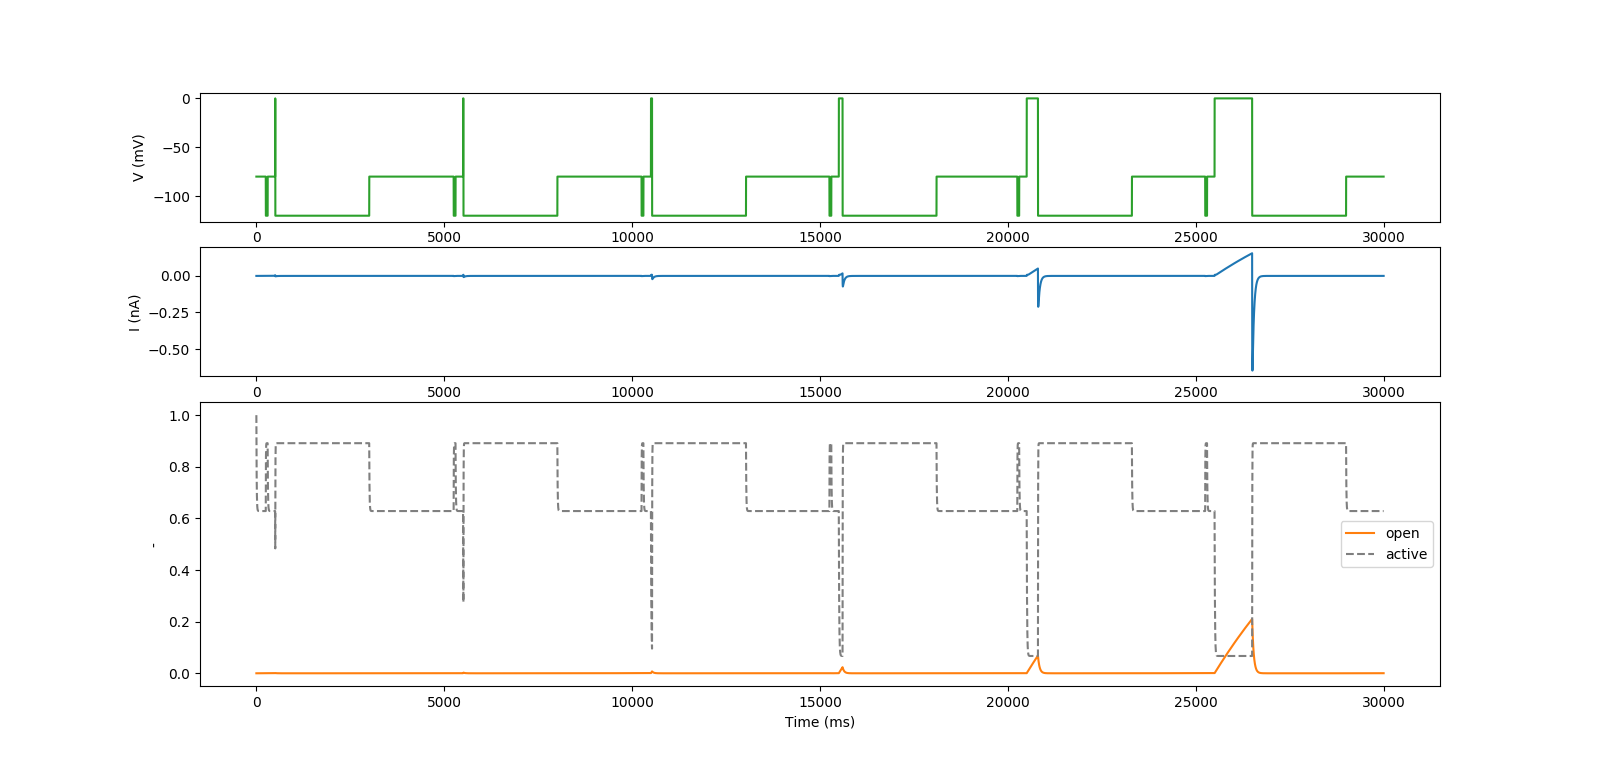
\includegraphics[width=0.95\textwidth]{fig/pr1-modified}
}
\caption{%
Pr1 (tidied)
}
\label{fig:analysis-pr1}
\end{figure}

% Analysis Pr2
\begin{figure}[H]
\centerline{
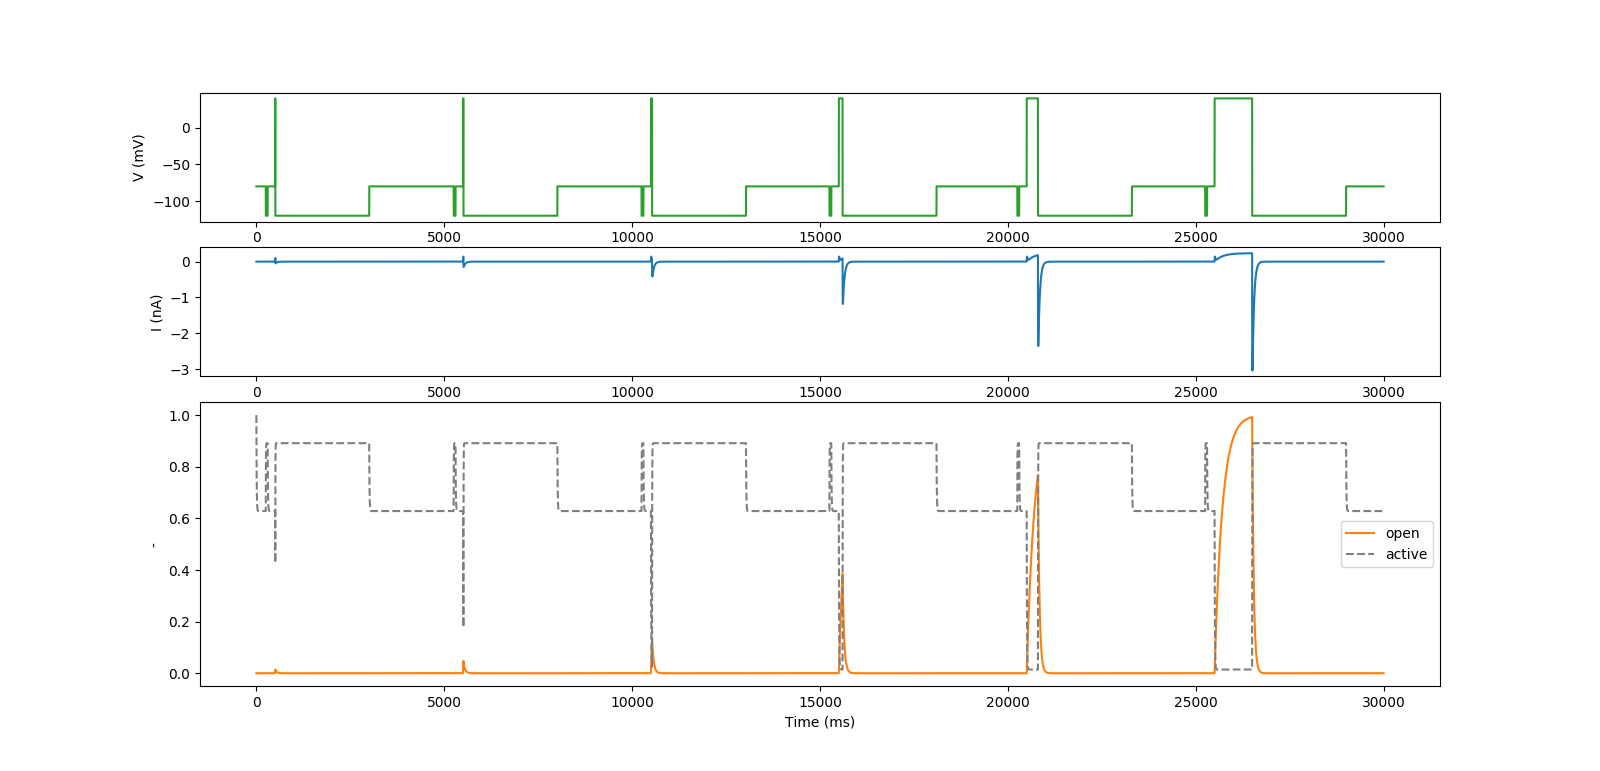
\includegraphics[width=0.95\textwidth]{fig/pr2-modified}
}
\caption{%
Pr2 (tidied)
}
\label{fig:analysis-pr2}
\end{figure}

Protocols are called ``activation kinetics 1 \& 2'', but what do they tell us
 about activation kinetics?
Overlaying the different steps shows the (voltage-dependent) activation takes
 the same course at every (same-voltage) step (but note this is a model
 prediction, and more complicated behaviour might occur if a more complicated
 model was used).

% Analysis Pr2
\begin{figure}[H]
\centerline{
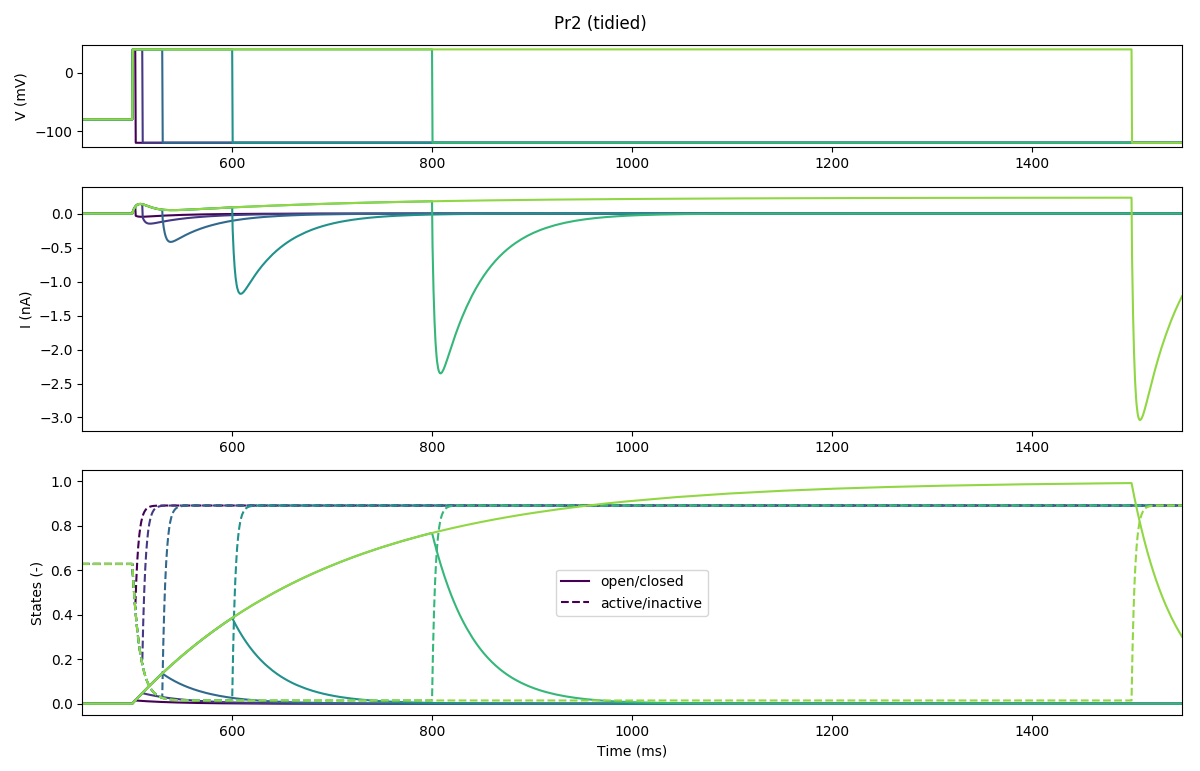
\includegraphics[width=0.95\textwidth]{fig/pr2-modified-folded}
}
\caption{%
Pr2 (tidied, steps overlayed).
Notice the currents at each step follow the same, slow upwards line, before
dropping down at the end of the step.
In other words, the activation is the same at each step (as expected given that
they step to the same voltage, from the same pre-condition).
}
\label{fig:analysis-pr2-folded}
\end{figure}

As a result, the full trace of the longest step provides all information
 encoded in the shorter steps.
If we measure the current at the end of each step, this provides a low-sampling
 rate digitisation of the longest step.
The difference between Pr1 and Pr2 is the height of this step (0mV vs 40mV),
 so that effectively Pr1 and Pr2 give us bad digitisations of the activation
 process at two different voltages.

Both steps are preceded by the same sequence of a short time at -80mV, then
 -120mV (to measure leak), then back to -80mV.
Each repeat of the activation protocol Pr3 starts with the same sequence,
 followed by a very long (5s) step to several voltages, including 0mV and 40mV.
As a result, the activation protocol Pr3 contains the longest step from Pr1 and
 the longest step from Pr2.
So we can conclude that \emph{using whole-trace fitting, the information we aim
 to extract with Pr1 and Pr2 is already contained in Pr3}.

Other parts of Pr1 and Pr2 might be interesting for aspects other than
 activation (although from the figures above it does not seem to be the case).

%
% Pr1/2: Summary statistic
%
\subsubsection{Pr1/2: Summary statistic}

Pr1 can be used to derive 6 points of the activation curve for a step to 0mV,
 by taking the final value during the variable length step.
Pr1 can be used to derive 6 points of the activation curve for a step to 40mV,
 by taking the final value during the variable length step.

We can try it out in simulation:

% Simulation sum stat Pr1 and Pr2
\begin{figure}[H]
\centerline{
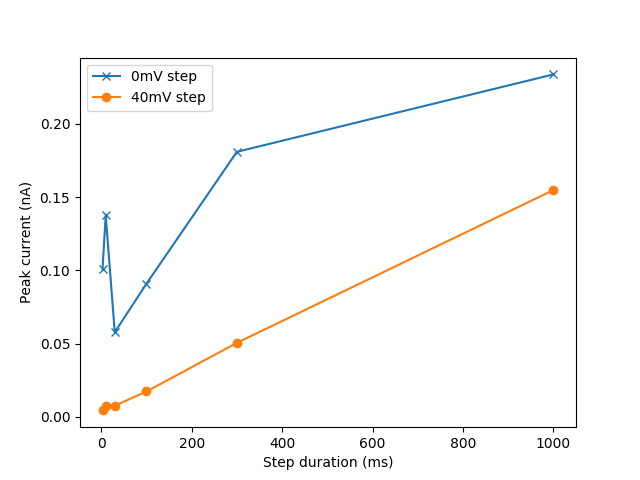
\includegraphics[width=0.5\textwidth]{fig/pr12-modified-stat}
}
\caption{%
Pr1 and Pr2 summary statistic:
Simulated peak current during variable step, versus step duration in Pr1 (0mV)
and Pr2 (+40mV).
}
\label{fig:analysis-pr12-stat}
\end{figure}

What happened here? To see why the lines are crooked near the start, we can
inspect our simulation results, specifically the first milliseconds of the
variable step:

% Simulation sum stat Pr1 and Pr2
\begin{figure}[H]
\centerline{
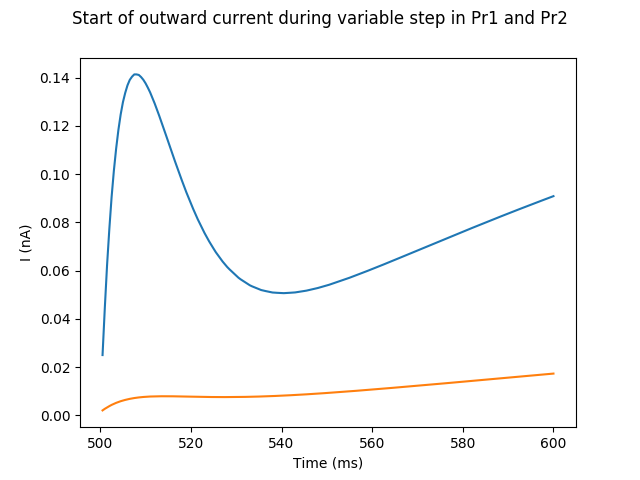
\includegraphics[width=0.5\textwidth]{fig/pr12-modified-step-start}
}
\caption{%
Current during first milliseconds of the longest variable step in Pr1 and Pr2.
}
\label{fig:analysis-pr12-step-start}
\end{figure}

So our model starts with a little hump, before settling into the gradual ascent
 more easily seen in the earlier figures.
Looking back at the states, this is the result of inactivation (a dip down from
 approximately 0.6 to zero).
Judging by its time course, this should affect the first 3 steps, which is
 borne out by the figure above.

\emph{If} this effect is seen in real cells (but e.g. \citet{Zhou1998IKrHERG}
 doesn't show it), then this is an issue for this protocol.

\subsubsection{Up for discussion}

1. The 3ms step in Pr1 and Pr2 is filtered out completely by the 5ms
capacitance filter.

2. Note that Kylie's paper says these protocols are \emph{shortened} (so that
 they could all be performed together on the same cell, with and without
 dofetilide).
So might need to add points for fairer comparison.
On the other hand, this way we can do everything on one cell, which is not
 usually done.

3. Another difference with a standard analysis is that this would use an
 average of multiple cells.
This might 'contaminate' the data with cell-to-cell variability, but could also
 reduce noise.
Perhaps it'd be best for us to take a few points near each point we want to
 measure (e.g. a few points of ``peak current'') and take the mean of those, to
 reduce the influence of noise.

%
% Pr1: Data from cell 5
%
\subsubsection{Pr1: Data from cell 5}

% Pr 1 cell 5
\begin{figure}[H]
\centerline{
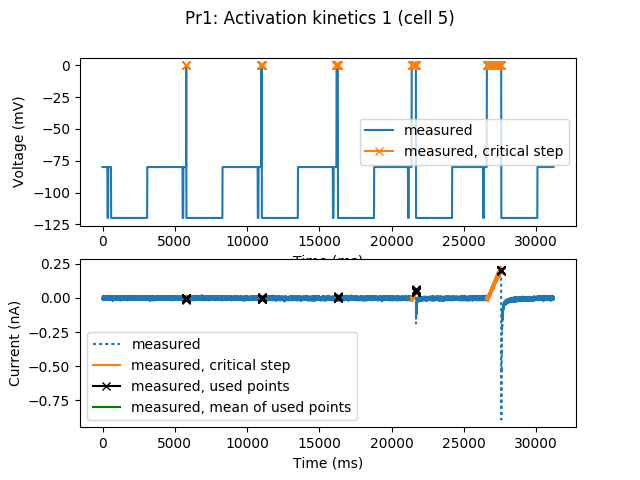
\includegraphics[width=0.5\textwidth]{fig/pr1-cell-5}
}
\caption{%
Current in cell 5 during Pr1
}
\label{fig:analysis-pr1-cell-5}
\end{figure}

\Fig{analysis-pr1-cell-5} shows that the real data isn't terribly exciting
during Pr1, except for the final two steps.
As noted above, the first step is even removed entirely by the capacitance
 filtering.
However, step 2 shows that nothing happens at this duration, so we probably
 don't need to worry about that.

% Pr 1 cell 5 zoom
\begin{figure}[H]
\centerline{
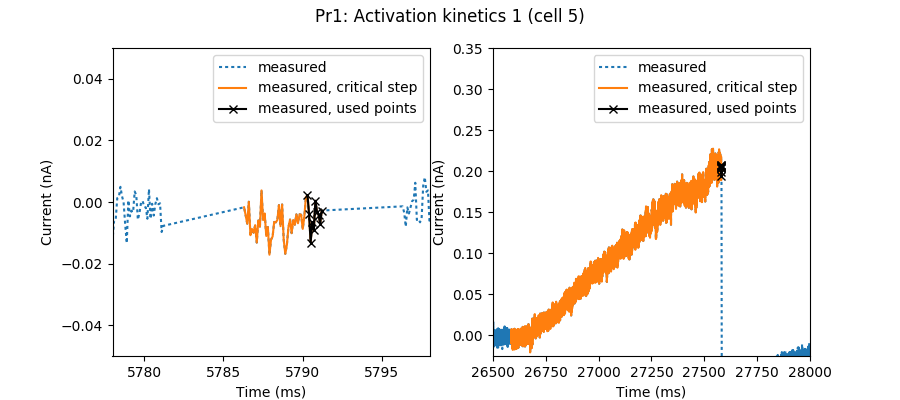
\includegraphics[width=0.95\textwidth]{fig/pr1-cell-5-zoom}
}
\caption{%
Current in cell 5 during Pr1, second and last step
}
\label{fig:analysis-pr1-cell-5-zoom}
\end{figure}

\Fig{analysis-pr1-cell-5-zoom} shows the second and last steps, with the parts
 used for the summary statistic highlighted.
Instead of using the final point in the trace, I took 10 points (1 $\micro$s)
 and took the mean.
As the right panel shows, this still doesn't look like a great estimate of
 where a line fit through the entire highlighted current would go.

% Pr 1 cell 5 summary stat
\begin{figure}[H]
\centerline{
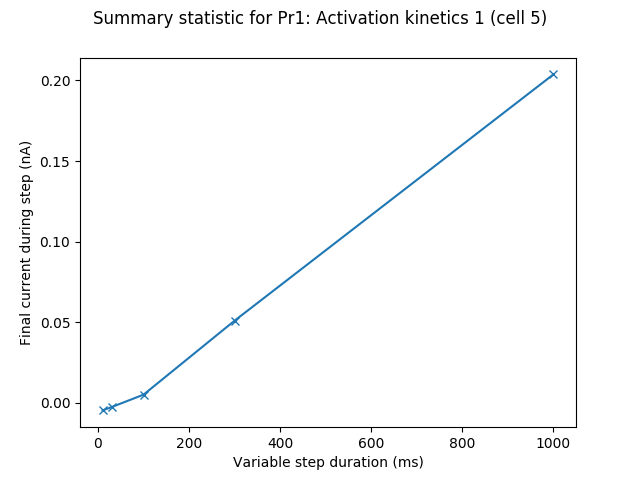
\includegraphics[width=0.95\textwidth]{fig/pr1-cell-5-statistic}
}
\caption{%
Summary statistic for Pr1 on Cell 5.
}
\label{fig:analysis-pr1-cell-5-statistic}
\end{figure}

%
% Pr1/2: Data from cell 5
%
\subsubsection{Pr1 and Pr2: Real vs simulated}

% Simulation sum stat Pr1 and Pr2
\begin{figure}[H]
\centerline{
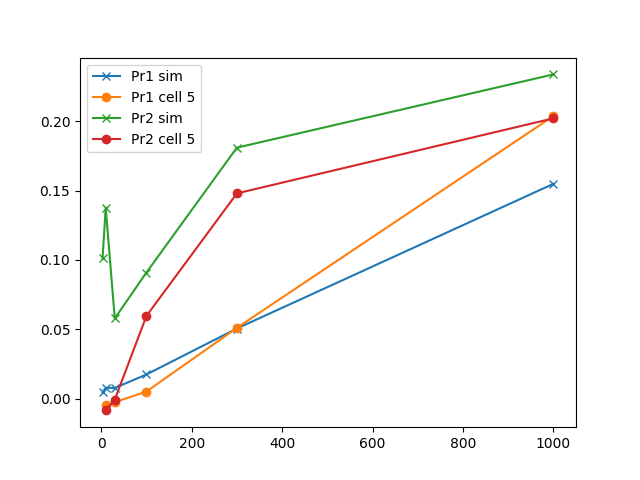
\includegraphics[width=0.5\textwidth]{fig/pr12-cell5-and-sim}
}
\caption{%
Pr1 and Pr2: Cell 5 data and simulation (with tidied protocol).
The longer steps are ok, but the lower steps show an artefact in the simulation
that's not observed in real cells.
}
\label{fig:pr12-cell5-and-sim}
\end{figure}

%
% Pr3: Steady-state activation
%
\subsection{Pr3: Steady-state activation}

% Analysis Pr3
\begin{figure}[H]
\centerline{
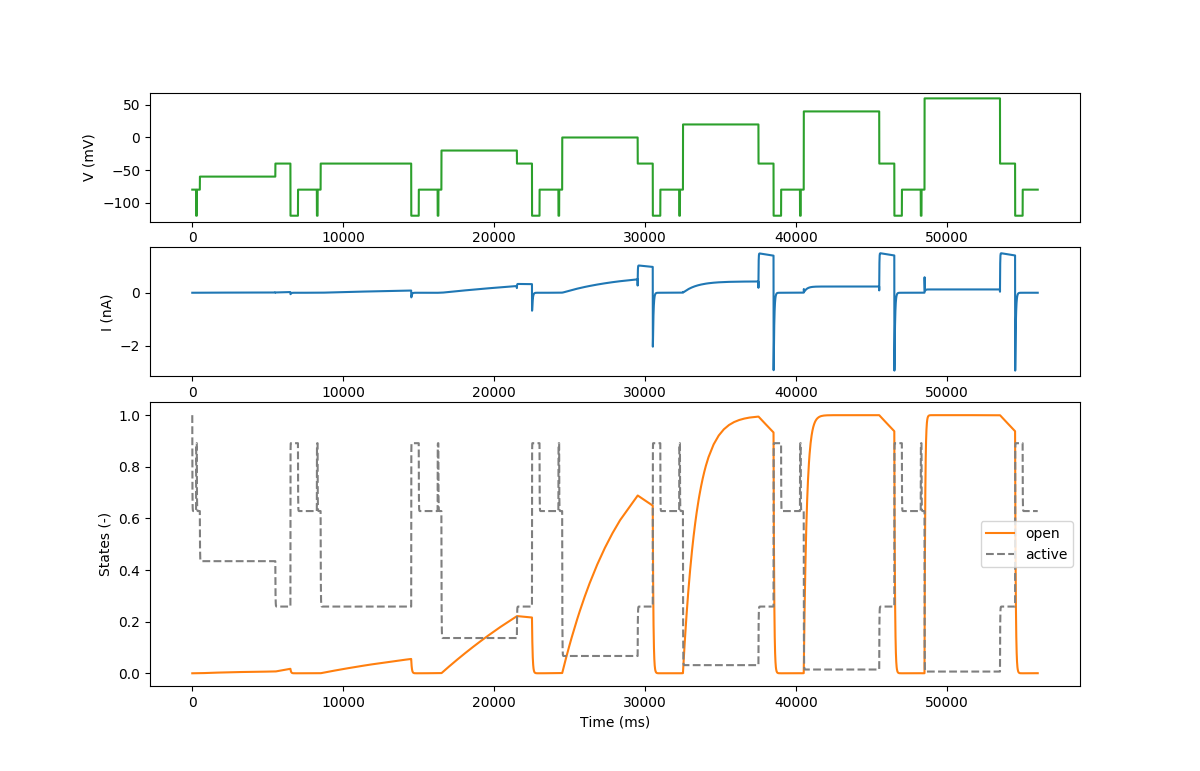
\includegraphics[width=0.95\textwidth]{fig/pr3-modified}
}
\caption{%
Pr3 (tidied)
}
\label{fig:analysis-pr3}
\end{figure}

This protocol does a good job of opening the channel, as \fig{analysis-pr3}
 shows.
This is good, as it creates some signal for us to observe.
It steps to a number of different voltages too, so we can get some voltage
 dependence info.

% Analysis Pr3 folded
\begin{figure}[H]
\centerline{
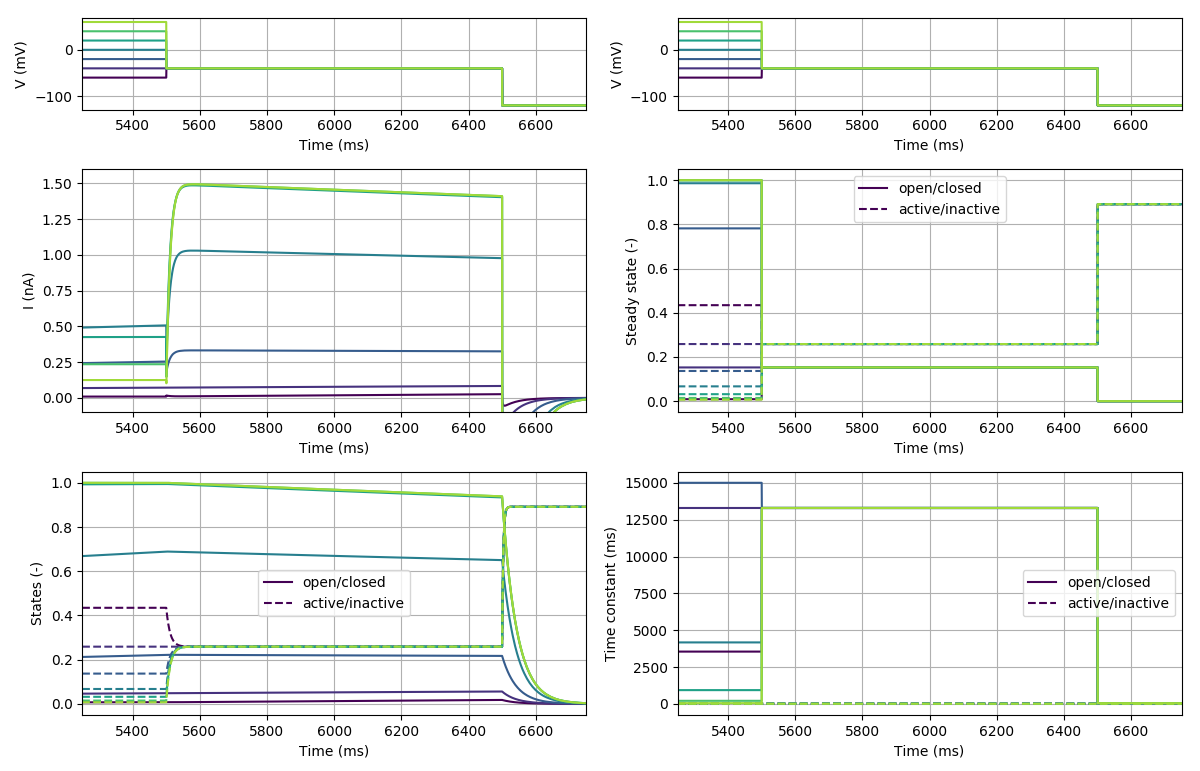
\includegraphics[width=0.95\textwidth]{fig/pr3-modified-folded}
}
\caption{%
Pr3 (tidied, steps overlayed). Simulated with Kylie's model using the
parameters obtained for the fit to the full traditional traces.
}
\label{fig:analysis-pr3-folded}
\end{figure}

The critical bit of the protocol is the step to -40mV \emph{after} the varying
 voltage step.
\Fig{analysis-pr3-folded} shows what happens during this step.
The current shown here is quite different from what is observed in real cells,
 see e.g. \citet{Sanguinetti1990IKIsIKrAndIKs}.

% Analysis Sanguinetti
\begin{figure}[H]
\centerline{
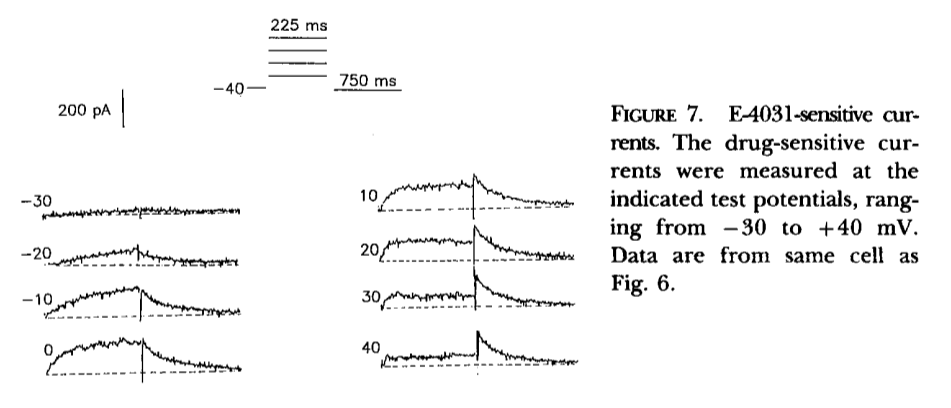
\includegraphics[width=0.95\textwidth]{fig/sanguinetti-1990-ikr-tail}
}
\caption{%
The first recording of IKr \citep{Sanguinetti1990IKIsIKrAndIKs}.
Note the immediate rise after the voltage step to -40mV (the tail current),
followed by exponential decay.
}
\label{fig:sanguinetti}
\end{figure}

\Fig{sanguinetti} shows the expected behaviour during this step: an
exponentially decreasing tail current, whose peak (right at the start of the
fixed-voltage step) can be measured.

% Analysis Pr3 folded TNNP
\begin{figure}[H]
\centerline{
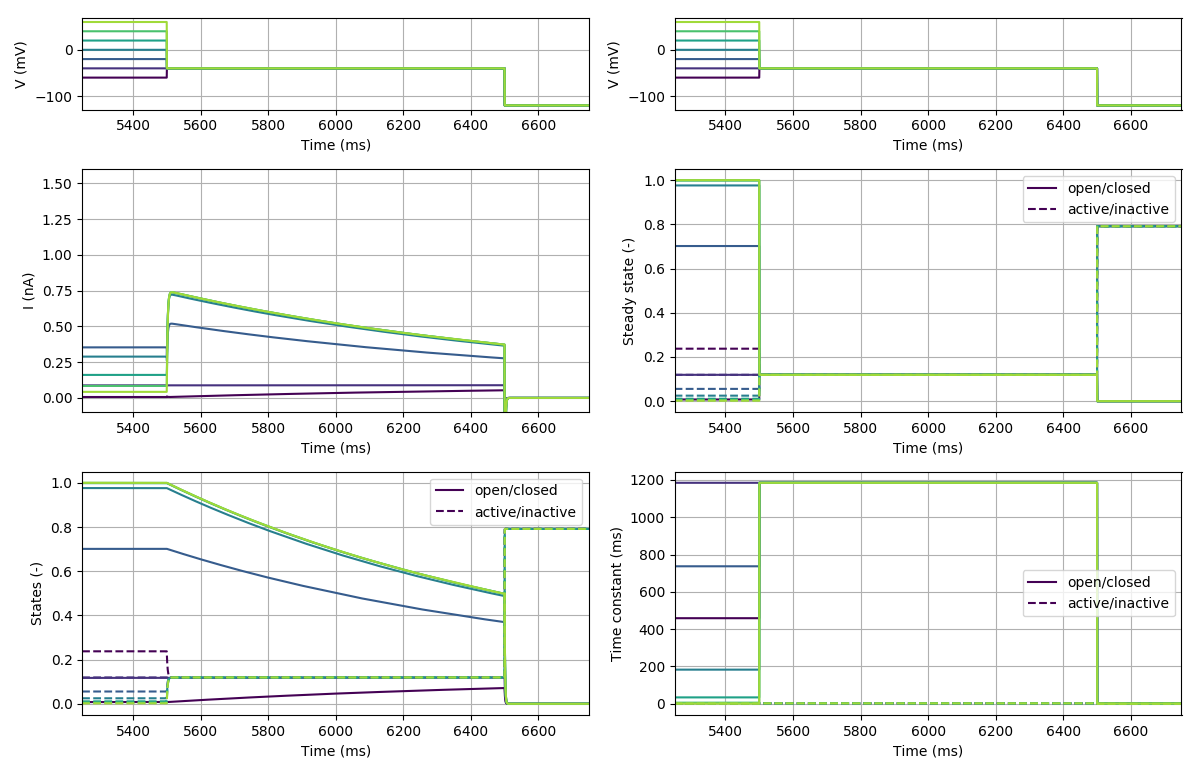
\includegraphics[width=0.95\textwidth]{fig/pr3-modified-folded-tnnp}
}
\caption{%
Pr3 (tidied, steps overlayed). Simulated with the \ikr\ model from
\citet{tenTusscher2006Model}.
}
\label{fig:analysis-pr3-tnnp}
\end{figure}

The model by \citet{tenTusscher2006Model} does show the (qualitatively) correct
behaviour, as shown in \fig{analysis-pr3-tnnp}.
The middle-right panel shows that, just before the step to -40mV, the
 open/closed state variable has its steady state at values ranging from 0mV to
 1mV.
This is good, as this is the variable we'd like to measure.
Upon the step to -40mV, inactivation immediatly kicks in (bottom left panel),
 because its time constant at this voltage is very small (bottom right panel).
The time constant for open/closed is much larger, so that the peak current
 during the -40mV has a fixed activation/inactivation (since it's all at -40mV)
 but a variable open/closed (since it's still at the value it obtained during
 the variable voltage step).
This means that, by normalising, we can get an estimate of the steady state of
 opening/closing.

Note however, that all this depends on the time-constants being just right!
What happens in the \fig{analysis-pr3-folded}?
First, it seems that the time constant of inactivation at -40mV is too large, so
that we can clearly see the rising current at the start of the -40mV, instead of
the near instantaneous jump in \fig{sanguinetti} and \fig{analysis-pr3-tnnp}.
Second, the time constant of opening/closing is 10 times larger than in the
 TNNP model, leading to the very slow decay after the peak.
So for the behaviour \emph{is} there, just time-scaled beyond recognition.

Note that the TNNP model uses a tricky formulation that separates the
steady-states and time constants (basing one on an $\alpha$ and $\beta$ but
specifying the other independently).
Perhaps for similar reasons?
It could be that a two-state HH model is not able to correctly reproduce this
behaviour (at least not when parametrised to also capture other desired
behaviours).

%
% Pr3: Summary statistic
%
\subsection{Pr3: Summary statistic}

%
% Pr3 in cell 5
%
\subsection{Pr3 in cell 5}

Interestingly, cell 5 showed the same `unexpected' behaviour as the simulations
based on the full-trace cell 5 fits.

% Analysis Pr3 cell 5
\begin{figure}[H]
\centerline{
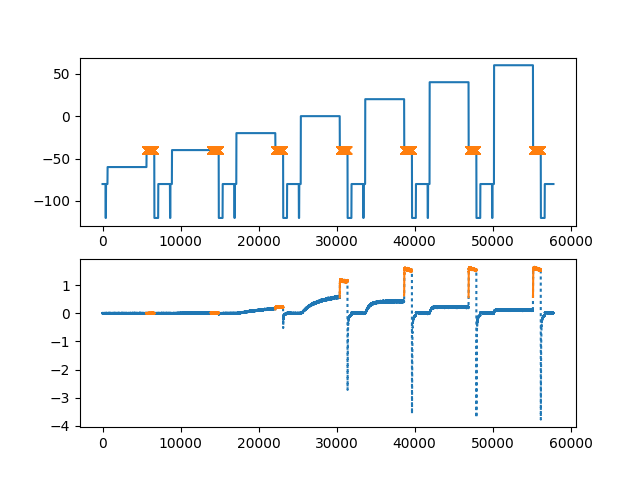
\includegraphics[width=0.5\textwidth]{fig/pr3-cell-5}
}
\caption{%
Pr3 in cell 5.
}
\label{fig:analysis-pr3-cell-5}
\end{figure}

Zooming in, we can clearly see the slow rise at the start of the step, and the
subsequent decay is so slow that the noise obscured the true peak location.

% Analysis Pr3 cell 5 zoom
\begin{figure}[H]
\centerline{
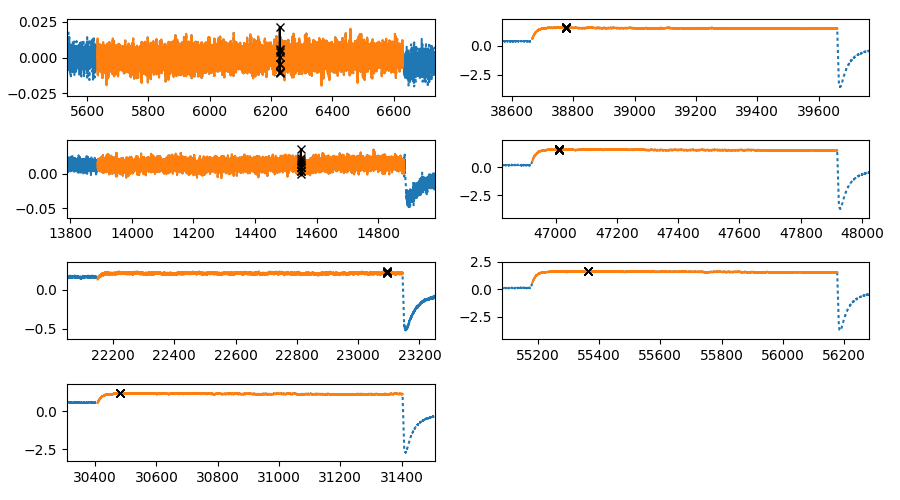
\includegraphics[width=0.95\textwidth]{fig/pr3-cell-5-zoom}
}
\caption{%
Pr3 in cell 5, zoomed in on the critical steps.
}
\label{fig:analysis-pr3-cell-5-zoom}
\end{figure}

Is this perhaps due to the lower temperature (21-22 deg C in Kylie's data,
versus 35 in \citet{Sanguinetti1990IKIsIKrAndIKs} and the
\citet{Zhou1998IKrHERG} data that the model by \citet{tenTusscher2006Model} is
based on.

% Zhou tail current at 23 and 35
\begin{figure}[H]
\centerline{
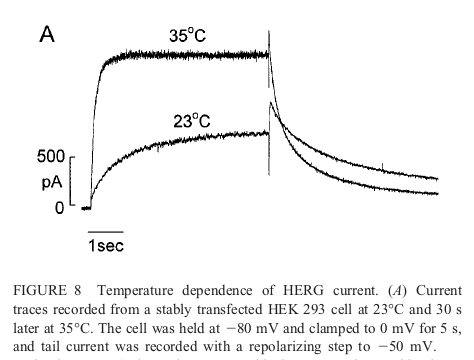
\includegraphics[width=0.95\textwidth]{fig/zhou-ikr-tail-temperature}
}
\caption{%
IKr (HERG) tail current in a HEK cell at 23 and 35 deg C, from
\citep{Zhou1998IKrHERG}.
}
\label{fig:zhou-ikr-tail-temperature}
\end{figure}

\Fig{zhou-ikr-tail-temperature} shows that this could be partially the case.

IDEA

Ultimately, this is all another argument in favour of not using a HH style
 analysis that depends on assumptions about the time constants of the system
 you're about to measure!
Maybe that's the best argument actually, regardless of quality of fit,
 signal-to-noise ratios, analysis differences, etc.
The analysis \& protocol \emph{can} depend on pre-existing knowledge of the
 system, in a way they must, and optimal design certainly assumes so.
\emph{But} they should be robust against large variations in the parameters we
 aim to discover.
\emph{Especially} in the light of biological variability, not to mention drug
 block, mutations and other instances where we actually want to \emph{show}
 that the parameters have changed.
We should maybe think of some way to measure how well our protocols work over
 wide ranges of possible parameters


%
%
% Comparing
%
%
\section{Comparing different types of fitting}

%
% AP validation
%
\subsection{AP validation}

Comparing methods by looking at model prediction for AP signal.

Loaded protocol from matlab, cell 5 data from matlab.

\begin{figure}[H]
\centerline{
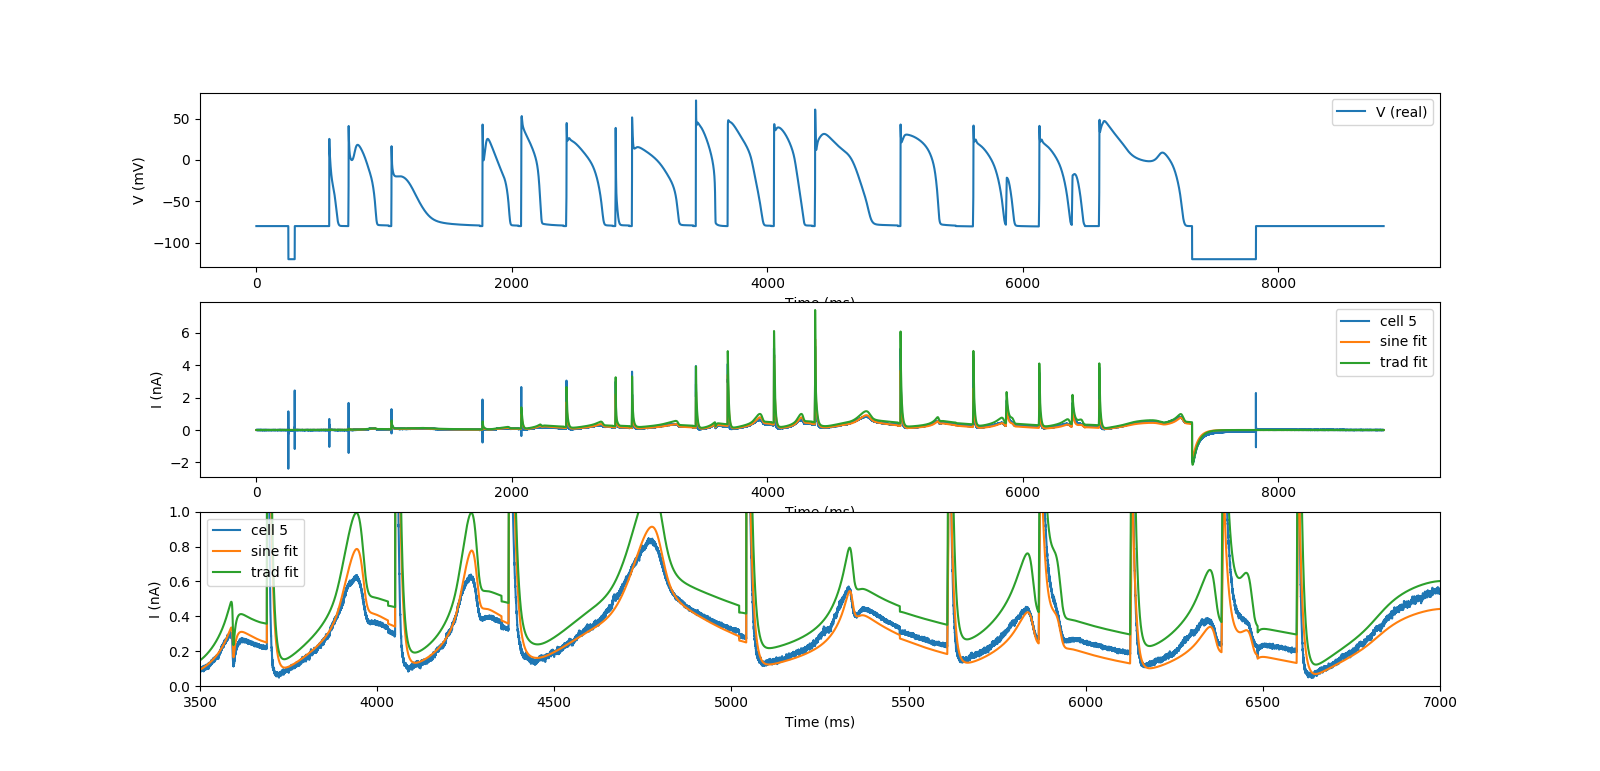
\includegraphics[width=0.95\textwidth]{fig/validation-ap-protocol}
}
\caption{%
AP protocol: Data from cell 5 plus simulation based on sine-wave fit
parameters and trad. prot. fit parameters.
}
\label{fig:validation-ap-protocol}
\end{figure}

\begin{table}[H]
\centering
\caption{%
AP protocol validation log-likelihoods.
}
\label{tab:validation-ap-protocol}
\startrowcolors
\footnotesize
\begin{tabular}{ll}
\hline
\thead{Fit} & \thead{Log-posterior} \\
\hline
Sine wave   & -21273679.167 \\
Trad. prot. & -74641604.9933 \\
\hline
\end{tabular}
\end{table}



%
% Sine-wave validation
%
\subsection{Sine-wave cross-validation}

\begin{figure}[H]
\centerline{
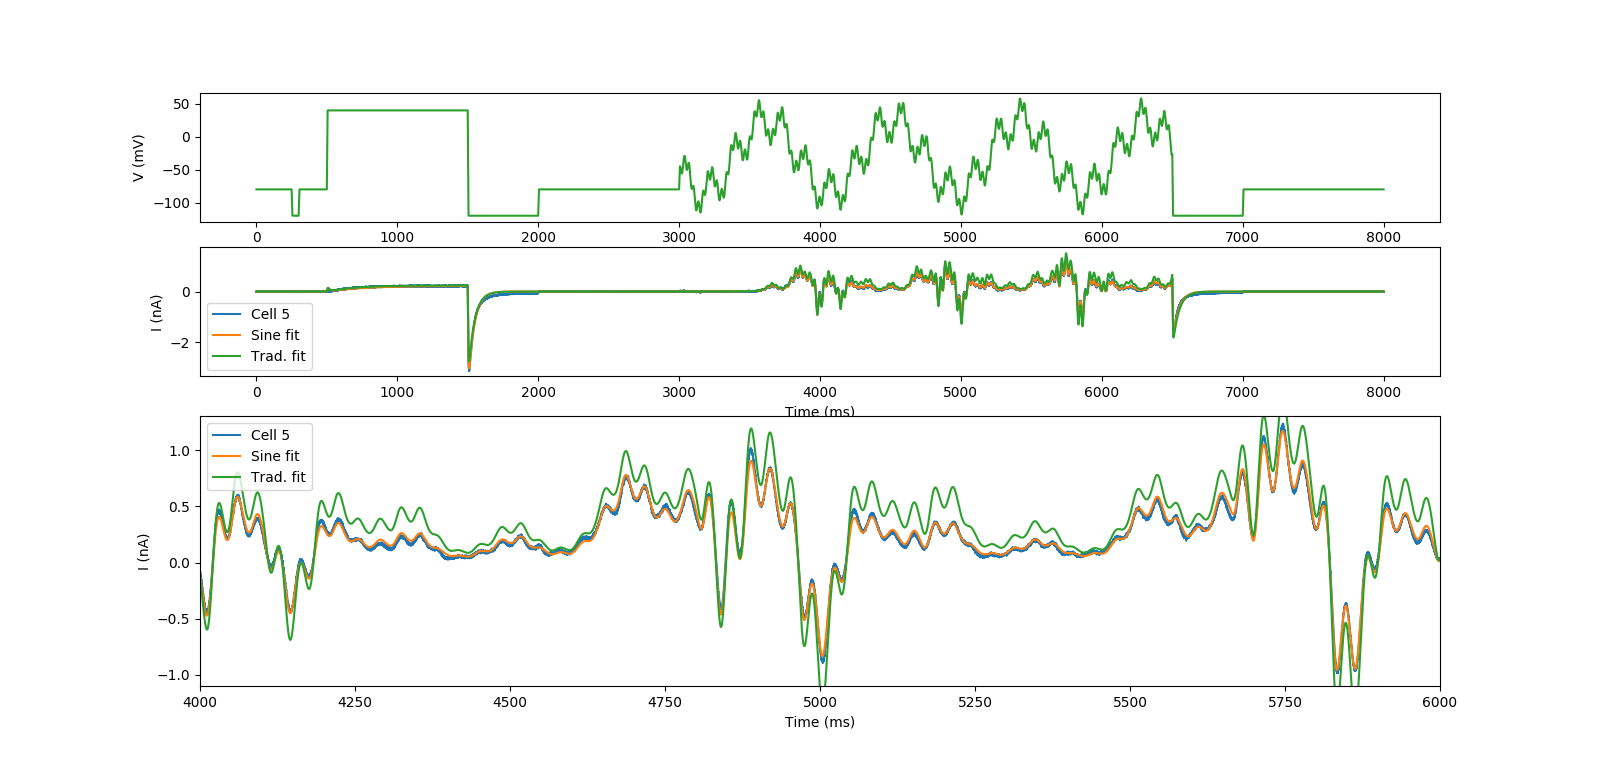
\includegraphics[width=0.95\textwidth]{fig/validation-sine-wave}
}
\caption{%
Sine-wave protocol: Data from cell 5 plus simulation based on sine-wave fit
parameters and trad. prot. fit parameters.
}
\label{fig:validation-sine-wave}
\end{figure}

\begin{table}[H]
\centering
\caption{%
Sine wave validation log-likelihoods.
}
\label{tab:validation-sine-wave}
\startrowcolors
\footnotesize
\begin{tabular}{ll}
\hline
\thead{Fit} & \thead{Log-posterior} \\
\hline
Sine wave   & -1509487.67775 \\
Trad. prot. & -18791120.0047 \\
\hline
\end{tabular}
\end{table}

% Validation Pr1
\begin{figure}[H]
\centerline{
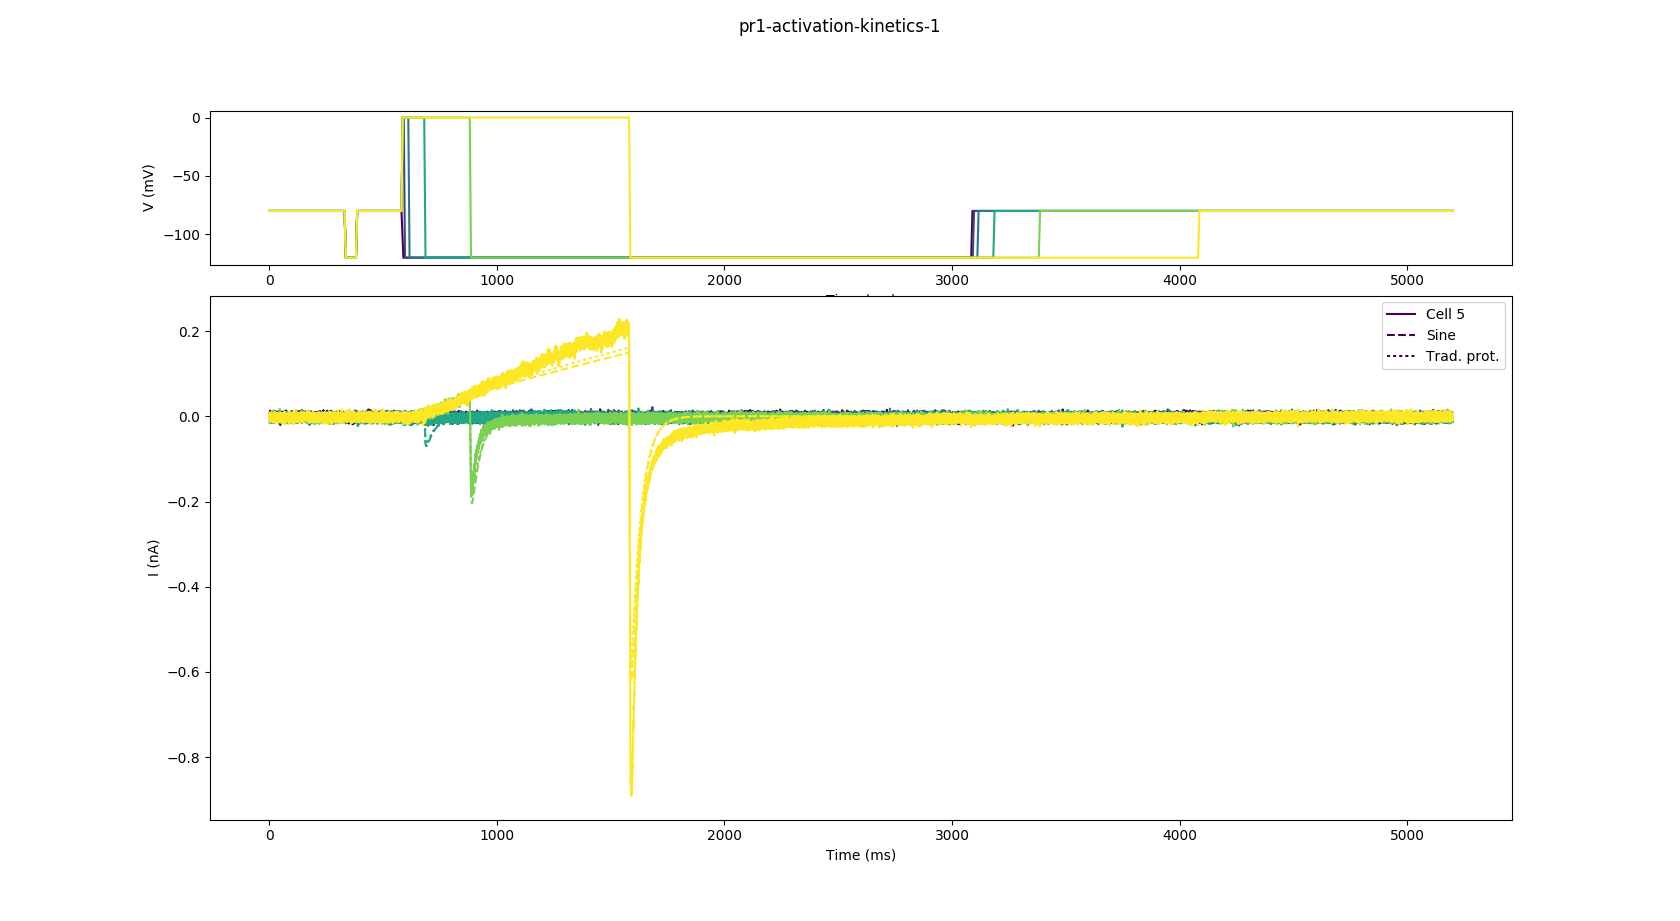
\includegraphics[width=0.95\textwidth]{fig/validation-pr1}
}
\caption{%
Pr1
}
\label{fig:validation-pr1}
\end{figure}

% Validation Pr2
\begin{figure}[H]
\centerline{
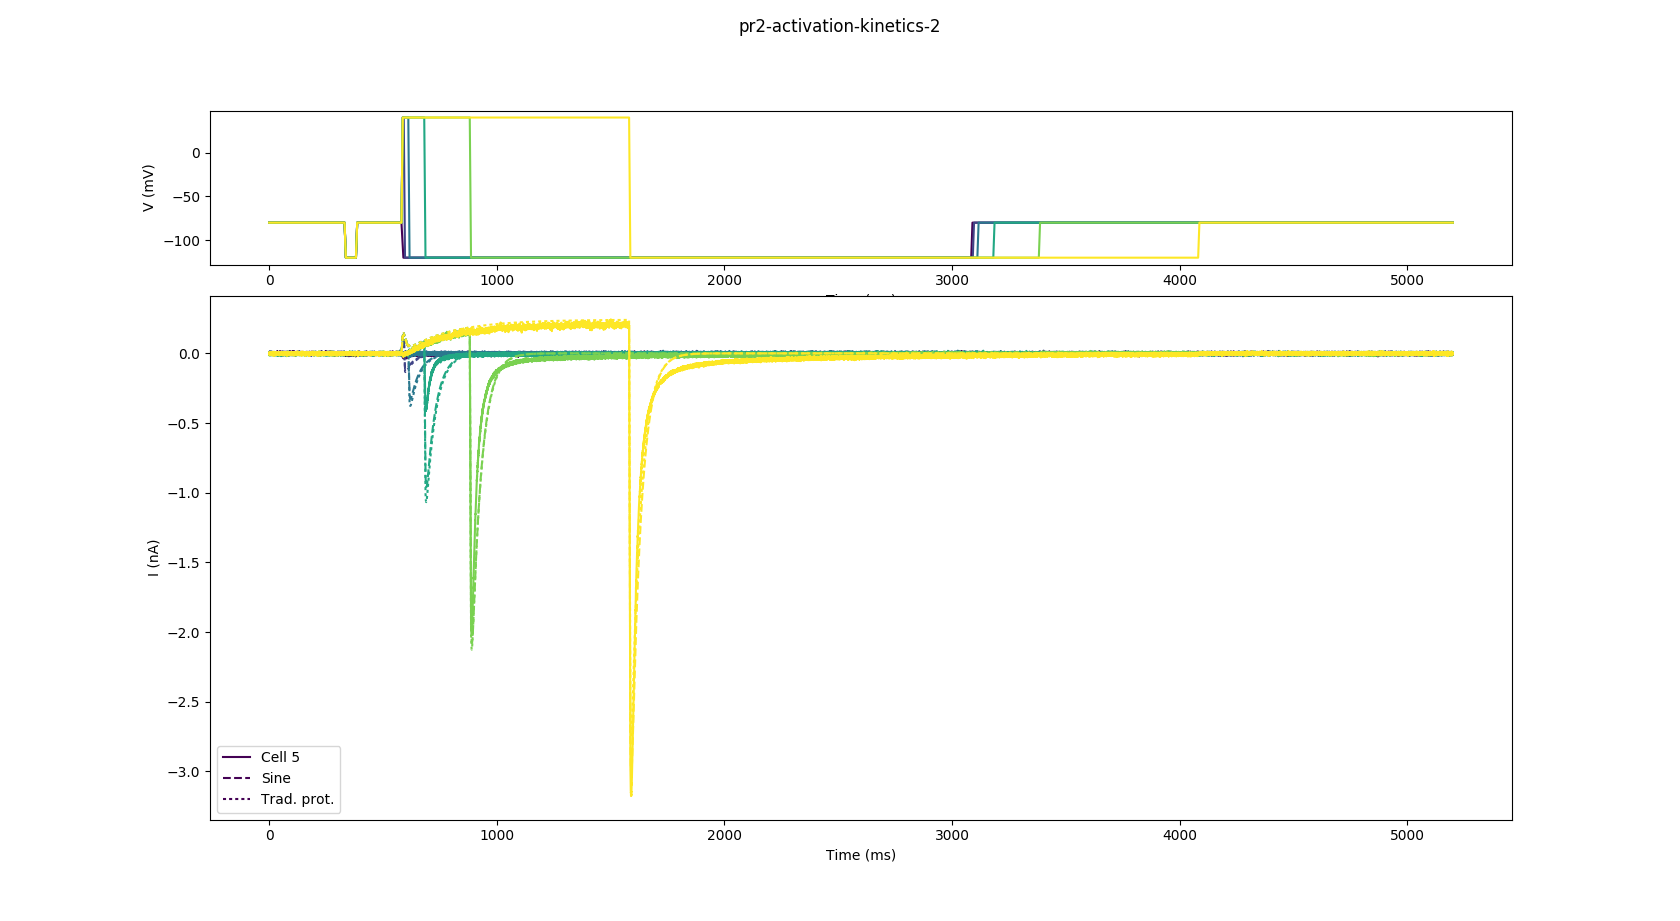
\includegraphics[width=0.95\textwidth]{fig/validation-pr2}
}
\caption{%
Pr2
}
\label{fig:validation-pr2}
\end{figure}

% Validation Pr3
\begin{figure}[H]
\centerline{
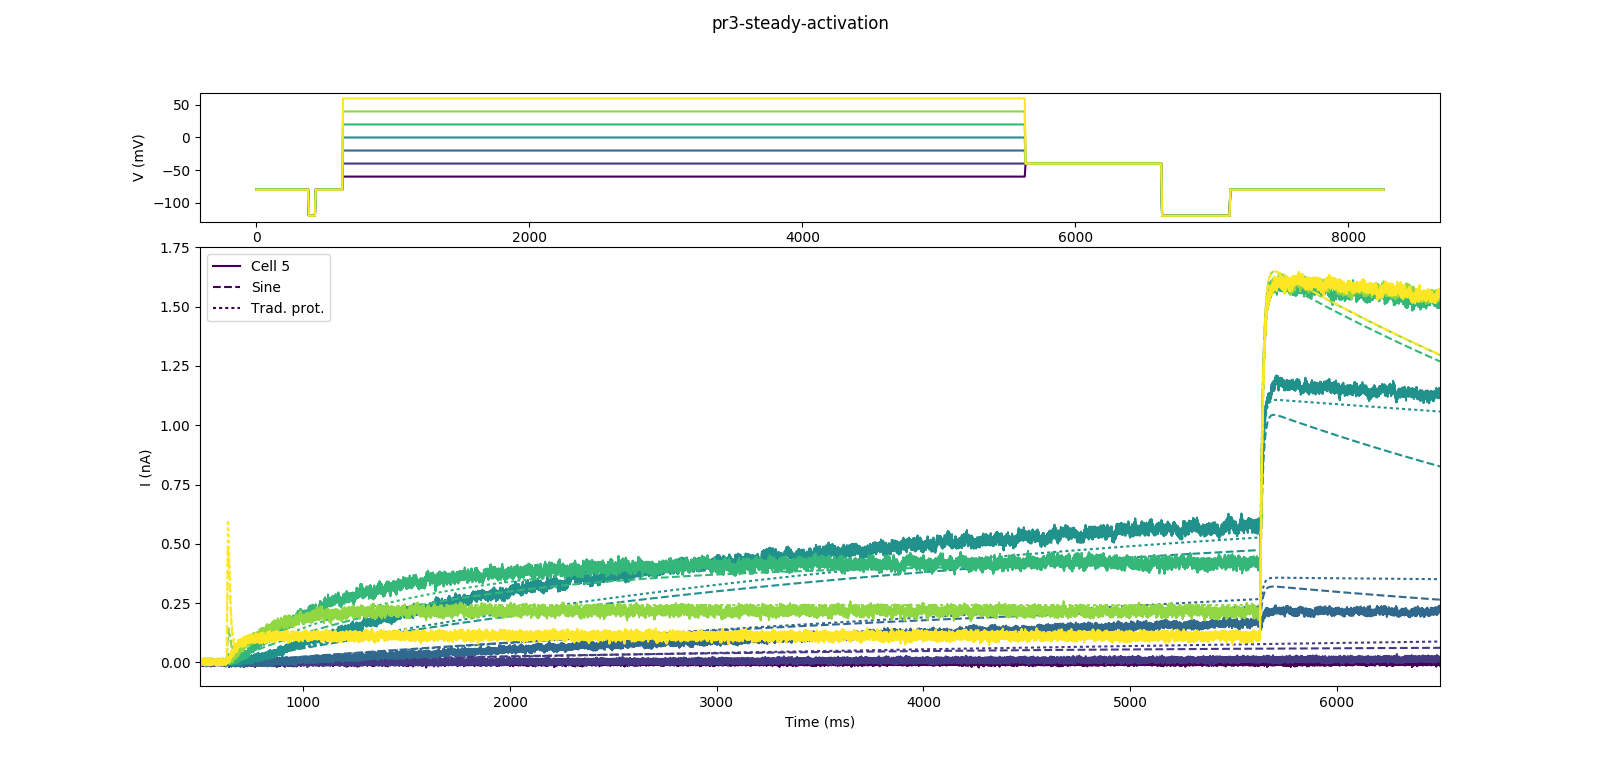
\includegraphics[width=0.95\textwidth]{fig/validation-pr3}
}
\caption{%
Pr3
}
\label{fig:validation-pr3}
\end{figure}

% Validation Pr4
\begin{figure}[H]
\centerline{
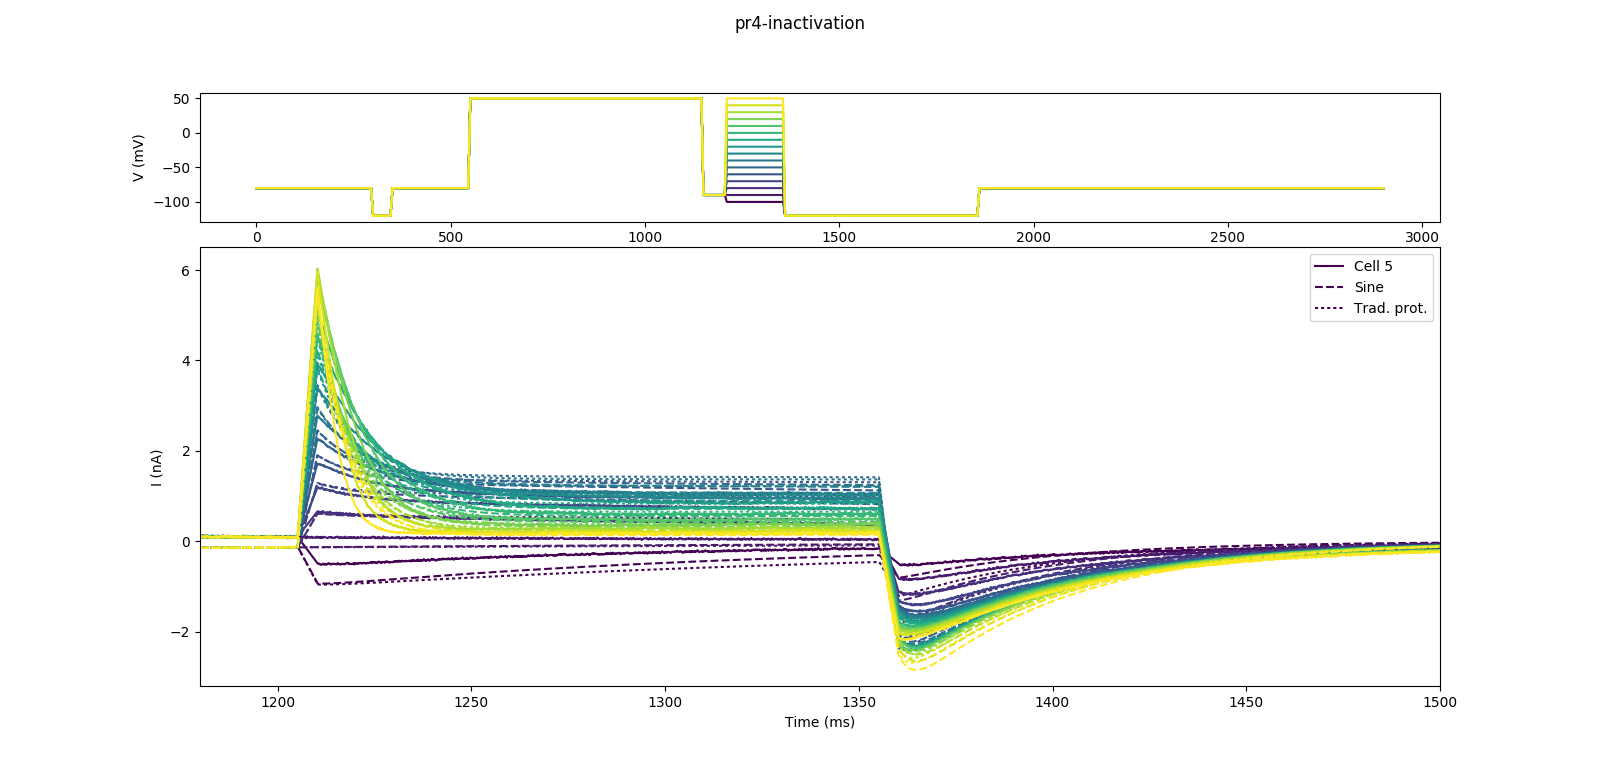
\includegraphics[width=0.95\textwidth]{fig/validation-pr4}
}
\caption{%
Pr4
}
\label{fig:validation-pr4}
\end{figure}

% Validation Pr5
\begin{figure}[H]
\centerline{
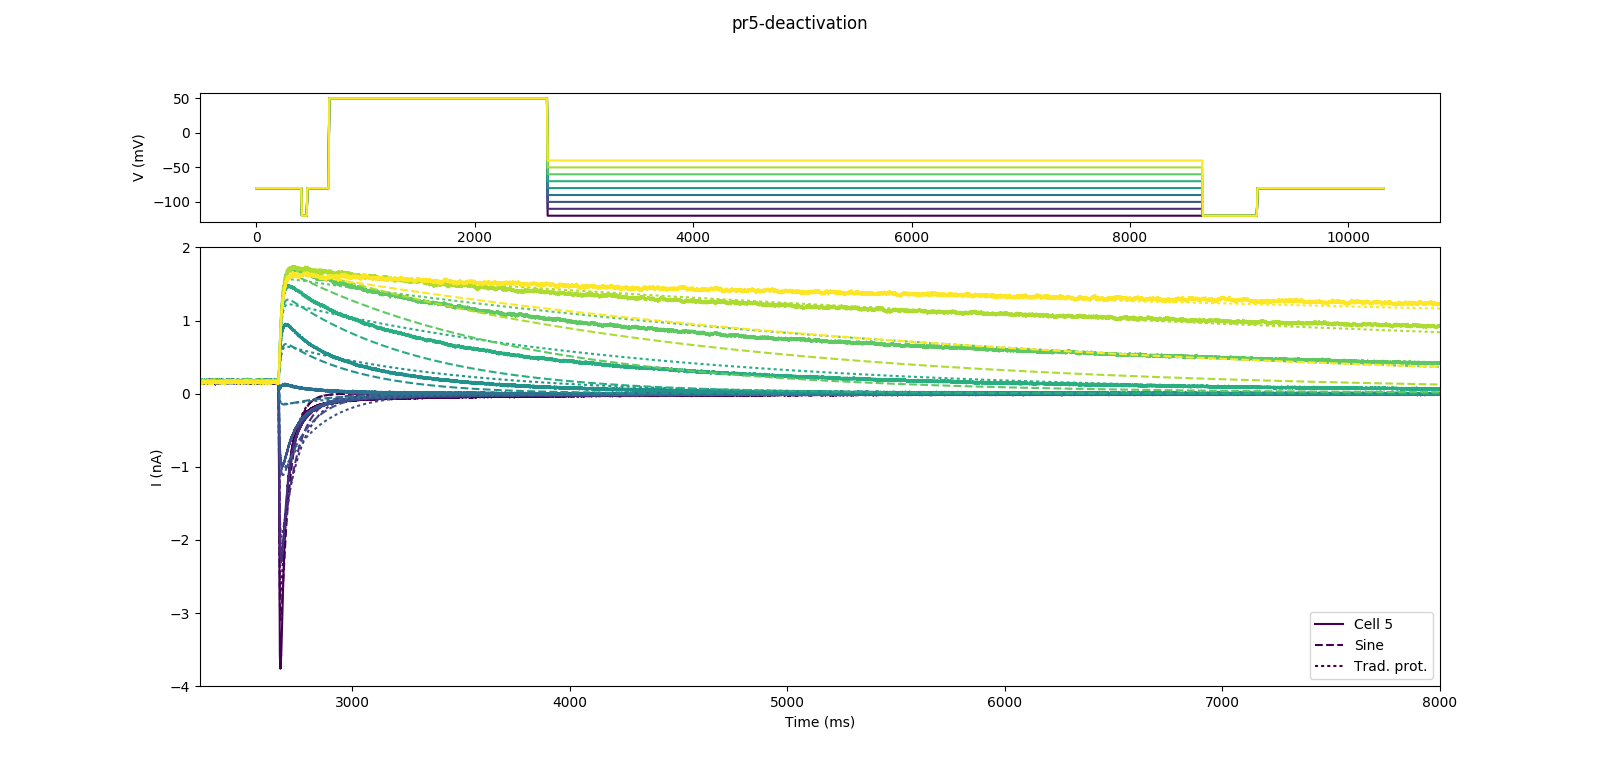
\includegraphics[width=0.95\textwidth]{fig/validation-pr5}
}
\caption{%
Pr5
}
\label{fig:validation-pr5}
\end{figure}




%
% Trad. prot. validation
%
\subsection{Trad. prot. cross-validation}

\begin{table}[H]
\centering
\caption{%
Trad. prot. validation log-likelihoods.
}
\label{tab:validation-trad-prot}
\startrowcolors
\footnotesize
\begin{tabular}{lll}
\hline
\thead{Prot.} & \thead{Fit} & \thead{Log-posterior} \\
\hline
Pr1 (ak-1)  & \textbf{sine} & 473746 \\
Pr1 (ak-1)  & trad          & 441919 \\
\hline
Pr2 (ak-2)  & \textbf{sine} & -6329912 \\
Pr2 (ak-3)  & trad          & -7443985 \\
\hline
Pr3 (s.act) & sine          & -80888280 \\
Pr3 (s.act) & \textbf{trad} & -39387497 \\
\hline
Pr4 (inact) & \textbf{sine} & -14161029 \\
Pr4 (inact) & trad          & -19444287 \\
\hline
Pr5 (deact) & sine          & -1188041457 \\
Pr5 (deact) & \textbf{trad} & -41635915 \\
\hline
\hline
Combined    & sine          & -1288946932 \\
Combined    & \textbf{trad} & -107469765 \\
\end{tabular}
\end{table}




































%
%
% Acknowledgments
%
%
%\section*{\Ack}

%A.C.D. was funded by the Rhodes Trust, UK.
%M.C., J.C., G.R.M. and D.J.G. acknowledge support from BBSRC grant BB/P010008/1.
%K.A.B was supported by the EPSRC grant numbers EP/I017909/1 and EP/K503769/1.
%This work was supported by the Wellcome Trust [grant number 101222/Z/13/Z]: G.R.M. gratefully acknowledges support from a Sir Henry Dale Fellowship jointly funded by the Wellcome Trust and the Royal Society.


%
%
% Supplement
%
%
\newpage
\appendix





%
%
% Problem statement
%
%
\section{Problem statement}
We have some noisy time-series data and a forward model (simulation) that can
 be used to replicate it.
We'd like to find out which parameter values are compatible with the
 experimental evidence.

\subsection{Single series}

\begin{enumerate}
\item Observations $D = \{(t_1, z_1),...,(t_n, z_n)\}$ where $t$ is time
 ($t_i > t_{i-1}$ for $i > 1$) and $z_i\in\real$ is a noisy measurement at
 time $t_i$.
\item Forward model $\mu(t|\theta) \to \real$ with $m$ parameters, bundled in
 $\theta$.
\item The parameters live in some bounded space
 $\theta\in\Theta\subset\real^m$
\item \emph{Only} normally distributed, time-independent noise with some
 unknown variance $\sigma^2$, such that
 $z_i = \mu(t_i|\theta_{true}) + \normal(0, \sigma^2)$.
\end{enumerate}

Numbers 1,2,3 are definitions.
Number 4 is a dodgy assumption that we'll revisit later.

For the single series problem, we can now define the \emph{likelihood} of a
 parameter set $\theta$ as the probability \emph{density} of obtaining
 observations $D$ for parameters $\theta$:
\begin{equation}
l(\theta|D) \equiv f(D|\theta)
\end{equation}
With our dodgy assumption of purely random noise, the measurement error at any
 point in time is independent of the signal history, so that:
\begin{equation}
f(D|\theta) = \prod_{i=1}^{n} f(t_i,z_i|\theta)
\end{equation}
With normally distributed noise, the probability density function for
 observing $D$ is then:
\begin{equation}
f(x|\theta,\sigma) = \prod_{i=1}^{n} \frac{1}{\sqrt{2\pi\sigma^2}}
    \exp \left(
        -\frac{\left(x_i - \mu(t_i|\theta)\right)^2}{2\sigma^2}
    \right)
\end{equation}
And taking the logarithm, we find
\begin{equation}
\log l(\theta,\sigma|D) =
    - \frac{n}{2} \log(2\pi)
    - n \log(\sigma)
    - \frac{1}{2\sigma^2} \sum_{i=1}^n \left(z_i - \mu(t_i|\theta) \right)^2
\end{equation}



\subsubsection{The value of sigma}

There are two strategies for finding $\sigma$:

\begin{enumerate}
\item Find a flat bit of signal, and use the sample standard deviation.
\item Add $\sigma$ to the parameter vector $\theta$.
\end{enumerate}



\subsubsection{Influence of sampling rate}

Assuming the noise is truly stochastic, we can double the sampling rate (so
 that a new point is inserted between any two subsequent points) and get more
 random noise.

\begin{equation}
\log l(\theta,\sigma|D) =
    - \frac{n}{2} \log(2\pi)
    - n \log(\sigma)
    - \frac{1}{2\sigma^2} \sum_{i=1}^n \left(z_i - \mu(t_i|\theta) \right)^2
\end{equation}

This will double the first two terms, and - if the original number of samples
 was large - approximately double the last term as well.

This seems wrong.
Ideally, we'd have some way to calculate the likelihood that would give a very
 wide distribution on $\theta$ for a low $n$, and then get more narrow as $n$
 decreases, \emph{until it stabilises at the point where the signal contains
 enough information}.
On the other hand, the more specific we are about exactly what random noise
 signal we measure, the less likely this exact result should become, so from
 the point of view of quantifying the likelihood of some random noise it makes
 sense...



\subsubsection{Relation to optimisation problems}

Given the loglikelihood equation
\begin{equation}
\log l(\theta,\sigma|D) =
    - \frac{n}{2} \log(2\pi)
    - n \log(\sigma)
    - \frac{1}{2\sigma^2} \sum_{i=1}^n \left(z_i - \mu(t_i|\theta) \right)^2
\end{equation}

Since $n$ and $\sigma$ are properties of the signal, indepdent of the model, we
 can treat the optimisation problem as minimising

\begin{equation}
\sum_{i=1}^n \left(z_i - \mu(t_i|\theta) \right)^2
\end{equation}

Similarly, we could start from the root-mean squared error (RMSE), which is
 basically the sample standard deviation (with $n$ instead of $n-1$:

\begin{equation}
\text{RMSE} = \sqrt{\frac{\sum_{i=1}^n \left(z_i - \mu(t_i|\theta) \right)^2}{n}}
\end{equation}

and this would give the same result.



\subsection{Combining multiple traces}

Following the dodgy assumption
\begin{equation}
f(D|\theta) = \prod_{i=1}^{n} f(t_i,z_i|\theta)
\end{equation}
combining traces can be achieved by simply adding more points to $D$.
(Another way to think about it would be to split a single series in 2, and work
 out what should happen knowing that the result should be unchanged).

More generally, we can look at the general MCMC problem

\begin{equation}
f(\theta|D) = \frac{f(D|\theta)f(\theta)}{f(D)}
\end{equation}

and add a second data set:

\begin{equation}
f(\theta|D,E) = \frac{f(D,E|\theta)f(\theta)}{f(D,E)}
\end{equation}

if $D$ and $E$ are independent, this becomes

\begin{equation}
f(\theta|D,E) = \frac{f(D|\theta)f(E|\theta)f(\theta)}{f(D,E)}
\end{equation}

so we can replace the likelihood in our original problem by the product of two
independent likelihoods!

For dependent $D$ and $E$ we'd have to solve

\begin{equation}
f(\theta|D,E) = \frac{f(D|E,\theta)f(E|\theta)f(\theta)}{f(D,E)}
\end{equation}

since we can't universally define $f(D|E,\theta)$ there's no point trying to do
this in a general way in Pints (though users can always hack it in).

But what about weighting?
Is there any reason we should?
For example, if we care about $n$, it may make sense to weigh by $1/n_i$ for
 each experiment $i$?

Making the link to miminising errors, it looks like we can just add up errors
then, unless we care about $n$.






%
% Distributions aren't obvious
%
\section{Distributions}

Following \citet{Papoulis2002Probability}.

Let $\bm{x}$ be a random variable

\begin{equation}
F(x) \equiv P\{\bm{x} \leq x\}
\end{equation}

then

\begin{align}
F(-\infty) &= 0 \\
F(+\infty) &= 1
\end{align}

\begin{flalign}
& x_1 < x_2 \rightarrow F(x_1) \leq F(x_2) \\
& F(x_0) = 0, x < x_0 \rightarrow F(x) = 0
\end{flalign}

\begin{flalign}
\{\bm{x} \leq x_2\} &= \{\bm{x} \leq x_1\} \cup \{x_1 < \bm{x} \leq x_2\} \\
P\{\bm{x} \leq x_2\} &= P\{\bm{x} \leq x_1\} + P\{x_1 < \bm{x} \leq x_2\} \\
P\{x_1 < \bm{x} \leq x_2\} &= P\{\bm{x} \leq x_2\} - P\{\bm{x} \leq x_1\} \\
                           &= F(x_2) - F(x_1)
\end{flalign}

if also

\begin{align}
F(x^+) &\equiv \lim_{\epsilon \downarrow 0} F(x + \epsilon) \\
F(x^-) &\equiv \lim_{\epsilon \uparrow 0} F(x + \epsilon)
\end{align}

then

\begin{align}
F(x_2) - F(x_1^-) = P\{x_1 \leq \bm{x} \leq x_2 \}
\end{align}

%
% PDFs
%
\subsection{Probability density functions}

Definition:
\begin{align}
f(x) \equiv \frac{d}{dx}F(x)
\end{align}
and
\begin{align}
\int_{-\infty}^{+\infty} f(x)dx = 1
\end{align}

\begin{align}
F(x) = \int_{-\infty}^{x} f(x)dx
\end{align}

\begin{align}
P\{x_1 < \bm{x} \leq x_2\} = F(x_2) - F(x_1) = \int_{x_1}^{x_2} f(x)dx
\end{align}

See \citet{Papoulis2002Probability} page 81.

%
% Independent PDFs
%
\subsubsection{Independent PDFs}

Vector of random variables
\begin{align}
\bm{X} = \{ \bm{x}_1, \bm{x}_2, ..., \bm{x}_n \}
\end{align}

\begin{align}
F(\bm{X}) = F(\{ \bm{x}_1, \bm{x}_2, ..., \bm{x}_n \}) = P\{\bm{x}_1 \leq x_1, \bm{x}_2 \leq x_2, ..., \bm{x}_n \leq x_n\}
\end{align}

PDF
\begin{align}
f(X) &\equiv \frac{\partial^n F(x_1, x_2, ..., x_n)}{\partial x_1 \partial x_2 \cdots \partial x_n}
\end{align}

\begin{align}
P\{\bm{X} \in D\} = \int_D f(X)dX, \qquad X = [x_1, x_2, ..., x_n]
\end{align}

where $D$ is a region (some volume).

For \emph{independent variables}:

\begin{align}
F(x_1, x_2, ..., x_n) &= F(x_1) F(x_2) \cdots F(x_3) \\
\frac{\partial}{\partial x_j} F_{i \neq j} &= 0
\end{align}
\begin{equation}
f(X)  = f(x_1) f(x_2) \cdots f(x_n)
\end{equation}

%
% Simple conditional PDFs
%
\subsection{PDFs conditional on an event}

\begin{align}
F(x_1 | A) = P\{\bm{x} \leq x_1 | A\} = \frac{P\{\bm{x} \leq x_1, A\}}{P(A)}
\end{align}

\begin{flalign}
& F(-\infty | A) = 0 \\
& F(+\infty | A) = 1 \\
& P\{x_1 < \bm{x} \leq x_2 | A\} = F(x_2|A) - F(x_1|A) \\
\end{flalign}

\begin{equation}
f(x|A) \equiv \frac{d}{dx} F(x | A)
\end{equation}

See \citet{Papoulis2002Probability} page 98.

Bayes rule

\begin{equation}
f(x|A) = \frac{P(A|\bm{x} = x)f(x)}{P(A)}
\end{equation}

See \citet{Papoulis2002Probability} page 103.

%
% Proper conditional PDFs
%
\subsection{PDFs conditional on a random variable}

\begin{align}
F(x | M) = P\{\bm{x} \leq x | M\} = \frac{P\{\bm{x} \leq x, M\}}{P(M)}
\end{align}

\begin{align}
F(x, y | M) = P\{\bm{x} \leq x, \bm{y} \leq y | M\} = \frac{P\{\bm{x} \leq x, \bm{y} \leq y, M\}}{P(M)}
\end{align}

We can use this to find the definition of

\begin{align}
F(y | x) \equiv F\{y | \bm{x} = x\}
\end{align}

by setting $M = \{x_1 < x \leq x_2\}$ and using some sneaky limits

\begin{equation}
F_y(y | x_1 < \bm{x} \leq x_2)
    = \frac{P\{x_1 < \bm{x} \leq x_2, \bm{y} \leq y\}}{P\{x_1 < \bm{x} \leq x_2\}}
    = \frac{F(x_2,y) - F(x_1,y)}{F_x(x_2) - F_x(x_1)}
\end{equation}

Take $\frac{\partial}{\partial y}$ to find

\begin{equation}
f_y(y | x_1 < \bm{x} \leq x_2)
    = \frac{\int_{x_1}^{x_2} f(x, y)dx}{F_x(x_2) - F_x(x_1)}
\end{equation}

Now set $x_1 = x$ and $x_2 = x + \Delta x$:

\begin{equation}
f_y(y | x < \bm{x} \leq x + \Delta x)
    = \frac{\int_{x}^{x + \Delta x} f(\alpha, y)d\alpha}{F_x(x + \Delta x) - F_x(x)}
\end{equation}

where
$ \int_{x}^{x + \Delta x} f(\alpha, y)d\alpha \approx f(x, y) \Delta x $
and
$ \frac{F_x(x + \Delta x) - F_x(x)}{\Delta x} \approx f_x(x) $

so that

\begin{equation}
f_y(y | x < \bm{x} \leq x + \Delta x)
    = \frac{\int_{x}^{x + \Delta x} f(\alpha, y)d\alpha}{F_x(x + \Delta x) - F_x(x)}
    \approx \frac{f(x, y) \Delta x}{f_x(x) \Delta x}
\end{equation}

finally, take the limit to zero to find

\begin{equation}
f_y(y | \bm{x} = x)
    = \lim_{\Delta x \to 0} f_y(y | x < \bm{x} \leq x + \Delta x)
    = \frac{f(x, y)}{f_x(x)}
\end{equation}

If we drop the $f_x$ and $f_y$ notation (assuming that the ambiguous $f$ is
clear from context), this becomes:

\begin{align}\label{cond_pdfs}
f(y|x) = \frac{f(x, y)}{f(x)} \qquad f(x|y) = \frac{f(x, y)}{f(y)}
\end{align}

See \citet{Papoulis2002Probability} page 221.


%
% Bayes for PDFs
%
\subsection{Bayes again}

From equation \ref{cond_pdfs} we get:

\begin{align}
f(x, y) = f(y|x)f(x) = f(x|y)f(y)
\end{align}

\begin{align}
f(x|y) = \frac{f(y|x)f(x)}{f(y)}
\end{align}

See \citet{Papoulis2002Probability} page 224.

\subsection{Independent conditions}

\begin{align}
f(x|y,z) &= \frac{P(y,z|x)f(x)}{f(y,z)}
\end{align}

Assuming independence:

\begin{align}
f(x|y,z) &= \frac{f(y,z|x)f(x)}{f(y,z)} \\
         &= \frac{f(y|x)f(z|x)f(x)}{f(y)f(z)} \\
         &= \frac{f(y|x)f(z|x)f(x)}{f(y)f(z)} \frac{f(x)}{f(x)}\\
         &= \frac{f(y|x)f(x)}{f(y)}\frac{f(z|x)f(x)}{f(z)}\frac{1}{f(x)} \\
         &= \frac{f(x|y)f(x|z)}{f(x)}
\end{align}



%
%
% References
%
%
\bibliographystyle{model2-names}
\bibliography{references}

\end{document}
